\chapter{Mutual information and metacommunities}
\lbl{ch:mm}

From the viewpoint of information theory, there is a conspicuous omission
from this text so far.  Given a random variable $X$ taking values in a
finite set, we have a measure of the information associated with $X$:
its entropy $H(X)$.  But suppose that we are also given another
random variable $Y$, not necessarily independent of $X$, taking values in
another finite set.  If we know the value of $X$, how much information does
that give us about the value of $Y$?

For instance, $Y$ might be a function of $X$, in which case knowing the
value of $X$ gives complete information about $Y$.  Or, at the other
extreme, $X$ and $Y$ might be independent, in which case knowing the
value of $X$ tells us nothing about $Y$.  We would like to quantify the
dependence between the two variables.  The covariance and correlation
coefficients will not do, since they are usually only defined
for random variables taking values in $\R^n$; and while they can be defined
in greater generality, there is no definition for an arbitrary pair of
finite sets.

From the viewpoint of diversity measurement, there is also something
missing.  We know how to quantify the diversity of a single community.
But when we have several associated or adjacent communities~-- for instance,
the gut%
%
\index{gut microbiome}%
\index{microbial systems}
% 
microbiomes of healthy and unhealthy adults, or the aquatic life in areas
of different salinity\index{salinity} near the mouth of a river~-- some
natural questions present themselves.  How much variation is there between
the communities?  Which contribute most to the overall diversity?  Which
are most or least typical in the context of the system as a whole?  The
diversity measures discussed so far give no answers to such questions.

We will see that these two problems, one information-theoretic and one
ecological, have the same solution. 

Our starting point is the classical information-theoretic concept of mutual
information (a measure of the dependence between two random variables) and
the closely related concepts of conditional and joint entropy.  These are
introduced in Section~\ref{sec:mm-info}.  Then we take exponentials of all
these quantities, which produces a suite of meaningful measures of an
ecological metacommunity (large community) divided into smaller
subcommunities.  The two random variables in play here correspond to a
choice of species and a choice of subcommunity.  Some of the measures
reflect features of individual subcommunities (Section~\ref{sec:mm-sub}),
while others encapsulate information about the entire metacommunity
(Section~\ref{sec:mm-meta}).  We establish the many good logical properties
of these measures in Section~\ref{sec:mm-props}.

All of the entropies and diversities in this chapter can be reduced to
relative entropy (Section~\ref{sec:all-ent-rel}).  In the diversity case,
they are also usefully expressed in terms of value, in the sense of
Chapter~\ref{ch:value}.  Reducing the various metacommunity and
subcommunity measures to one single concept provides new insights into
their ecological meaning.

The diversity measures treated in this chapter are a very special case of
those introduced in work of Reeve%
%
\index{Reeve, Richard|(} 
% 
et al.~\cite{HPD}.  In the terminology of Chapter~\ref{ch:sim}, it is the
case $q = 1$ (no deformation) and $Z = I$ (no inter-species similarity).
The framework of Reeve et al.\ allows a general $q$ (variable emphasis on
rare or common species) and a general $Z$ (to model the varying
similarities between species).  Section~\ref{sec:beyond} is a sketch of the
development for a general $q$, the details of which lie outside the scope
of this book.


\section{Joint entropy, conditional entropy and mutual information}
\lbl{sec:mm-info}


Shannon entropy $H$ assigns a real number $H(\p)$ to each probability
distribution $\p$, but information theory also associates several
quantities with any \emph{pair} of probability distributions.  To organize
them, it is helpful to distinguish between two types of quantity:
those defined for a pair of distributions on the \emph{same} set, and those
defined for a pair of distributions on potentially \emph{different} sets.

We have already met two quantities of the first type: the relative entropy
$\relent{\p}{\vc{r}}$ and cross entropy $\crossent{\p}{\vc{r}}$ of two
distributions $\p$ and $\vc{r}$ on the same finite set
(Chapter~\ref{ch:rel}).  

We now introduce the standard information-theoretic quantities of the
second type.  The material in this section is all classical, and can be
found in texts such as Cover and Thomas (\cite{CoTh1}, Chapter~2) and
MacKay (\cite{MacKITI}, Chapter~8).  As usual, we only
consider probability distributions on \emph{finite} sets.  But it is
convenient to switch from the language of probability distributions to that
of random variables.%
%
\index{random!variable}

So, \femph{for the rest of this section}, we consider a random variable $X$
taking values in a finite set $\XX$, and another random variable $Y$ taking
values in a finite set $\YY$.  Assuming that $X$ and $Y$ have the same
sample space, we also have the random variable $(X, Y)$, which takes values
in $\XX \times \YY$.

Given $x \in \XX$ and $y \in \YY$, we write
$\Pr((X, Y) = (x, y))$ as $\Pr(X = x, Y = y)$.  We usually abbreviate
$\Pr(X = x)$ as $\Pr(x)$\ntn{Px}, etc.  Thus, by definition, $X$ and $Y$
are independent%
% 
\index{independent!random variables} 
% 
if and only if
\[
\Pr(x, y) = \Pr(x) \Pr(y)
\]
for all $x \in \XX$ and $y \in \YY$.  The 
% 
conditional%
%
\index{conditional probability} 
% 
probability of $x$ 
given $y$ is
\[
\Pr(x \given y)
=
\frac{\Pr(x, y)}{\Pr(y)},
\]
and is defined as long as $\Pr(y) > 0$.  

The \demph{Shannon%
%
\index{Shannon, Claude!entropy}%
\index{entropy!Shannon} 
%
entropy} of the random variable $X$ is the Shannon
entropy of its distribution:
\[
H(X) 
=
\sum_{x \csuch \Pr(x) > 0} \Pr(x) \log \frac{1}{\Pr(x)}.
\ntn{HRV}
\]
Here and below, the variable $x$ in summations is assumed to run over the
set $\XX$ unless indicated otherwise, and similarly for $y$ in $\YY$.

\subsection*{Joint entropy}

The general definition of the entropy of a random variable can
be applied to the random variable $(X, Y)$, giving
\[
H(X, Y)
=
\sum_{x, y \csuch \Pr(x, y) > 0}
\Pr(x, y) \log \frac{1}{\Pr(x, y)},
\ntn{jointent}
\]
the \demph{joint%
%
\index{joint entropy} 
% 
entropy} of $X$ and $Y$.

\begin{examples}
\lbl{egs:joint}
\begin{enumerate}
\item
\lbl{eg:joint-ind}
Suppose that $X$ and $Y$ are independent.  If $X$ has distribution $\p$ and
$Y$ has distribution $\vc{r}$ then $(X, Y)$ has distribution $\p \otimes
\vc{r}$, so 
\[
H(X, Y) = H(X) + H(Y)
\]
by Corollary~\ref{cor:ent-log}.  

\item 
\lbl{eg:joint-one}
Suppose that $\YY$ is a one-element set.  Then the distribution of $Y$ is
uniquely determined, $H(Y) = 0$, and $H(X, Y) = H(X)$.

\item
\lbl{eg:joint-equal}
Suppose that $\XX = \YY$ and $X = Y$.  Then $H(X, Y) = H(X) = H(Y)$.

\item
\lbl{eg:joint-det}
Generalizing the last two examples, let us say that $Y$ is
\demph{determined%
%
\index{determined by} 
% 
by} $X$ if for all $x \in \XX$ such that $\Pr(x) > 0$,
there is a unique $y \in \YY$ such that $\Pr(x, y) > 0$.  Writing this
element $y$ as $f(x)$, we then have $\Pr(x, f(x)) = \Pr(x)$, or
equivalently, $\Pr(f(x)\given x) = 1$.  The joint entropy is given by
% 
\begin{align*}
H(X, Y) &
=
\sum_{x, y \csuch \Pr(x, y) > 0} 
\Pr(x, y) \log \frac{1}{\Pr(x, y)}      \\
&
=
\sum_{x \csuch \Pr(x) > 0} \Pr(x) \log \frac{1}{\Pr(x)} \\
&
=
H(X).
\end{align*}
\end{enumerate}
\end{examples}


\subsection*{Conditional entropy}

The definitions of the conditional entropies $\condent{X}{Y}$ and
$\condent{Y}{X}$ and the mutual information $I(X; Y)$ are suggested by the
schematic diagram of Figure~\ref{fig:venn-info}.
% 
\begin{figure}
\centering
\lengths\setlength{\unitlength}{.8mm}%
\begin{picture}(120,45)
\cell{60}{25}{c}{\includegraphics[height=40\unitlength]{venn_shadedm}}
\cell{60}{0}{b}{$H(X, Y)$}
\cell{25}{35}{c}{$H(X)$}
\cell{95}{35}{c}{$H(Y)$}
\cell{39}{25}{c}{$\condent{X}{Y}$}
\cell{60}{25}{c}{$I(X; Y)$}
\cell{81}{25}{c}{$\condent{Y}{X}$}
\end{picture}
\caption{Venn diagram showing entropic quantities associated with a pair of
  random variables taking values in different sets: the Shannon entropies
  $H(X)$ and $H(Y)$, the joint entropy $H(X, Y)$, the conditional entropies
  $\condent{X}{Y}$ and $\condent{Y}{X}$, and the mutual information $I(X;
  Y)$.}
\lbl{fig:venn-info}
\end{figure}
% 
The diagram depicts the joint entropy $H(X, Y)$ as the union of the two
discs and $\condent{X}{Y}$ as the complement of the second disc in the
union.  This suggests:

\begin{defn}
The \demph{conditional%
%
\index{conditional entropy} 
% 
entropy} of $X$ given $Y$ is
\[
\condent{X}{Y} = H(X, Y) - H(Y).
\ntn{condent}
\]
\end{defn}

We now explore this definition.  For each $y \in Y$
such that $\Pr(y) > 0$, there is a random variable $X\given y$\ntn{givenRV}
taking values in $\XX$, with distribution
\[
\Pr\bigl( (X \given y) = x\bigr)
=
\Pr(x \given y)
\]
($x \in \XX$).  Like all random variables, it has an entropy, $H(X
\given y)$.  The name `conditional entropy' is explained by
part~\bref{part:cond-alts-cond} of the following result.

\begin{lemma}
\lbl{lemma:cond-alts}
\begin{enumerate}
\item
\lbl{part:cond-alts-exp}
$\displaystyle
\condent{X}{Y} = \sum_{x, y \csuch \Pr(x, y) > 0} \Pr(x, y) \log
\frac{1}{\Pr(x \given y)}$.
\item
\lbl{part:cond-alts-cond}
$\displaystyle
\condent{X}{Y} = \sum_{y \csuch \Pr(y) > 0} \Pr(y) H(X \given y)$.
\end{enumerate}
\end{lemma}

\begin{proof}
For~\bref{part:cond-alts-exp}, first note that $\Pr(y) = \sum_x \Pr(x, y)$
for each $y \in \YY$, and in particular, $\Pr(y) > 0$ if there exists an
$x$ such that $\Pr(x, y) > 0$.  Hence
% 
% \begin{align}
\begin{equation}
H(Y)    %&
% =
% \sum_{y \csuch \Pr(y) > 0} 
% \Biggl( \sum_x \Pr(x, y) \Biggr)
% \log \frac{1}{\Pr(y)}
% \nonumber       \\
% &
=
\sum_{x, y \csuch \Pr(x, y) > 0} \Pr(x, y) \log \frac{1}{\Pr(y)}.
\lbl{eq:ca-1}
\end{equation}
% \end{align}
% 
It follows that
% 
\begin{align*}
\condent{X}{Y}  &
=
\sum_{x, y \csuch \Pr(x, y) > 0} \Pr(x, y) \log \frac{1}{\Pr(x, y)}
-
\sum_{x, y \csuch \Pr(x, y) > 0} \Pr(x, y) \log \frac{1}{\Pr(y)}      
\nonumber       \\
&
=
\sum_{x, y \csuch \Pr(x, y) > 0} 
\Pr(x, y) \log \frac{\Pr(y)}{\Pr(x, y)} \\
&
=
\sum_{x, y \csuch \Pr(x, y) > 0} 
\Pr(x, y) \log \frac{1}{\Pr(x \given y)},
\end{align*}
% 
proving~\bref{part:cond-alts-exp}.  This in turn is equal to 
\[
\sum_{y \csuch \Pr(y) > 0} \Pr(y)
\sum_{x \csuch \Pr(x \given y) > 0} 
\Pr(x \given y) \log \frac{1}{\Pr(x \given y)}
=
\sum_{y \csuch \Pr(y) > 0} \Pr(y) H(X \given y),
\]
% 
proving~\bref{part:cond-alts-cond}.
\end{proof}

The conditional entropy $\condent{X}{Y}$ is, therefore, the expected
entropy of the conditional random variable $X \given y$ when $y$ is chosen
at random.  It follows that $\condent{X}{Y} \geq 0$, or equivalently, that
$H(X, Y) \geq H(Y)$.


\begin{examples}
\lbl{egs:cond}
Consider again the four scenarios of Examples~\ref{egs:joint}.
% 
\begin{enumerate}
\item
\lbl{eg:cond-ind}
Suppose that $X$ and $Y$ are independent.  Then by
Example~\ref{egs:joint}\bref{eg:joint-ind}, 
\[
\condent{X}{Y} = H(X),
\qquad
\condent{Y}{X} = H(Y).
\]
Knowing the value of $Y$ gives no information on the value of $X$, nor vice
versa.  This is the situation shown in
Figure~\ref{fig:venn-special}\hardref{(a)}.

\item 
\lbl{eg:cond-one}
Suppose that $\YY$ is a one-element set.  Then by
Example~\ref{egs:joint}\bref{eg:joint-one}, 
% 
\begin{align*}
\condent{X}{Y}  &
=
H(X, Y) - H(Y) = H(X),  \\
\condent{Y}{X}  &
=
H(X, Y) - H(X) = 0.
\end{align*}

\item
\lbl{eg:cond-equal}
Suppose that $\XX = \YY$ and $X = Y$.  By
Example~\ref{egs:joint}\bref{eg:joint-equal}, $\condent{X}{Y} = 0$.  This
is intuitively plausible: once we know the value of $Y$, we know the value
of $X$ with certainty, so its probability distribution is concentrated on a
single element and therefore has entropy $0$.  Similarly, $\condent{Y}{X} =
0$.

\item
\lbl{eg:cond-det}
More generally, suppose that $Y$ is determined by $X$
(Figure~\ref{fig:venn-special}\hardref{(b)}).  Then by
Example~\ref{egs:joint}\bref{eg:joint-det},
% 
\begin{align}
\condent{X}{Y}  & 
= 
H(X) - H(Y),
\lbl{eq:cond-det-diff}        \\
\condent{Y}{X}  &
=
0.
\nonumber
\end{align}
% 
Since $\condent{X}{Y} \geq 0$, we have
\[
H(Y) \leq H(X)
\]
whenever $Y$ is determined by $X$.
\end{enumerate}
\end{examples}

\begin{figure}
\centering
\lengths
\begin{picture}(120,35)
\cell{30}{20}{c}{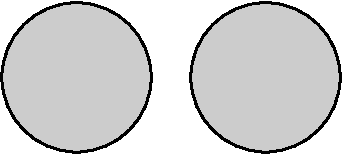
\includegraphics[width=50\unitlength]{venn_indm}}
\cell{100}{20}{c}{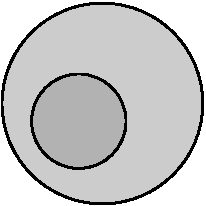
\includegraphics[width=30\unitlength]{venn_detm}}
% 
\cell{0}{31}{l}{$H(X)$}
\cell{55}{31}{c}{$H(Y)$}
\cell{30}{0}{b}{(a)}
% 
\cell{105}{25}{c}{$H(Y)$}
\cell{115}{32}{c}{$H(X)$}
\cell{100}{0}{b}{(b)}
\end{picture}
\caption{Venn diagrams for the cases in which \hardref{(a)}~the random
  variables $X$ and $Y$ are independent; \hardref{(b)}~$Y$ is determined by
  $X$.} 
\lbl{fig:venn-special}
\end{figure}

\begin{remark} 
\lbl{rmk:chain-rules}
In most texts, Lemma~\ref{lemma:cond-alts}\bref{part:cond-alts-cond} is
taken as the \emph{definition} of conditional entropy, and the equation
$\condent{X}{Y} = H(X, Y) - H(Y)$ that we took as our definition is proved
as a theorem.  This theorem is called the 
\demph{chain%
%
\index{chain rule!naming of}%
\index{chain rule!conditional entropy@for conditional entropy}
% 
rule}.  In other words, the chain rule states that
% 
\begin{equation}
\lbl{eq:joint-cond}
H(X, Y) 
=
H(Y) + \sum_{y \csuch \Pr(y) > 0} \Pr(y) H(X \given y).
\end{equation}
% 
It is essentially the same as what we have been calling the chain rule
throughout this text (beginning in Proposition~\ref{propn:ent-chain}).
This can be seen as follows.

Write $\XX = \{1, \ldots, k\}$ and $\YY = \{1, \ldots, n\}$.  Write $\vc{w}
= (w_1, \ldots, w_n) \in \Delta_n$ for the distribution of $Y$; thus, $w_i
= \Pr(Y = i)$ for each $i \in \YY$.  Also, for each $i \in \YY$ and $j \in
\XX$, define $p^i_j$ by
\[
w_i p^i_j = \Pr(X = j, Y = i),
\]
so that $\p^i = (p^i_1, \ldots, p^i_k) \in \Delta_k$ is the distribution of
the random variable $X \given i$.  (Here we have assumed that $\Pr(i) > 0$;
otherwise, choose $\p^i \in \Delta_k$ arbitrarily.)  Then $\vc{w} \of
(\p^1, \ldots, \p^n) \in \Delta_{nk}$ is the joint distribution of $X$ and
$Y$.  In this notation, equation~\eqref{eq:joint-cond} states that
\[
H\bigl( \vc{w} \of (\p^1, \ldots, \p^n) \bigr)
=
H(\vc{w}) + \sum_{i \csuch w_i > 0} w_i H(\p^i).
\]
This is exactly the chain rule in our usual sense.  
\end{remark}


\subsection*{Mutual information}

In Figure~\ref{fig:venn-info}, the intersection of the two discs is
labelled as $I(X; Y)$, and the inclusion-exclusion principle suggests the
formula
\[
H(X, Y) = H(X) + H(Y) - I(X; Y).
\]
We define $I(X; Y)$\ntn{mutinfo} to make this true:

\begin{defn}
The \demph{mutual%
%
\index{mutual information} 
% 
information} of $X$ and $Y$ is
\[
I(X; Y) = H(X) + H(Y) - H(X, Y).
\]
\end{defn}

Evidently $I$ is symmetric:
% 
\begin{equation}
\lbl{eq:mut-sym}
I(X; Y) = I(Y; X).
\end{equation}
% 
Alternative expressions for $I$, in terms of conditional rather than joint
entropy, follow immediately from the definitions and are also suggested by
the Venn diagram:
% 
\begin{equation}
\lbl{eq:mut-alt}
I(X; Y) = H(X) - \condent{X}{Y} = H(Y) - \condent{Y}{X}.
\end{equation}
% 
Mutual information can be expressed in two further ways still:

\begin{lemma}
\lbl{lemma:mut-alts}
\begin{enumerate}
\item 
\lbl{part:mut-alts-exp}
$\displaystyle
I(X; Y) = \sum_{x, y \csuch \Pr(x, y) > 0} 
\Pr(x, y) \log \frac{\Pr(x, y)}{\Pr(x) \Pr(y)}$.

\item
\lbl{part:mut-alts-mean-rel}
$\displaystyle
I(X; Y) = \sum_{y \csuch \Pr(y) > 0} \Pr(y) 
\relEnt{(X \given y)}{X}$.
\end{enumerate}
\end{lemma}

The right-hand side of~\bref{part:mut-alts-mean-rel} refers to the 
random variables $X \given y$ and $X$ taking values in $\XX$, and the
relative entropy of the first with respect to the second.

\begin{proof}
For~\bref{part:mut-alts-exp}, we have
% 
\begin{align*}
I(X; Y) &
=
H(X) - \condent{X}{Y}   \\
&
=
\sum_{x, y \csuch \Pr(x, y) > 0} \Pr(x, y) \log \frac{1}{\Pr(x)}
-
\sum_{x, y \csuch \Pr(x, y) > 0} \Pr(x, y) \log \frac{\Pr(y)}{\Pr(x, y)},
\end{align*}
% 
by equation~\eqref{eq:ca-1} and
Lemma~\ref{lemma:cond-alts}\bref{part:cond-alts-exp}.  Collecting terms,
the result follows.

To prove~\bref{part:mut-alts-mean-rel}, we use~\bref{part:mut-alts-exp} and
the equation $\Pr(x, y) = \Pr(y) \Pr(x \given y)$:
% 
\begin{align*}
I(X; Y) &
=
\sum_{x, y \csuch \Pr(y) > 0, \, \Pr(x \given y) > 0}
\Pr(y) \Pr(x \given y) \log\frac{\Pr(x \given y)}{\Pr(x)}       \\
&
=
\sum_{y \csuch \Pr(y) > 0} \Pr(y) 
\relEnt{(X \given y)}{X},
\end{align*}
% 
as required.
\end{proof}

The formula in~\bref{part:mut-alts-mean-rel} can be interpreted as
follows.  For probability distributions $\p$ and $\vc{r}$ on the same
finite set, $\relent{\p}{\vc{r}}$ can be understood as the information
gained when learning that the distribution of a random variable is $\p$,
when one had previously believed that it was $\vc{r}$.  Thus, $\relent{(X
  \given y)}{X}$ is the information gained about $X$ by learning that $Y =
y$.  Consequently,
\[
\sum_{y \csuch \Pr(y) > 0} \Pr(y) \relent{(X \given y)}{X}
\]
is the expected information about $X$ gained by learning the value of $Y$.
This is the mutual information $I(X; Y)$.  Briefly put, it is the
information that $Y$ gives about $X$.

For instance, if $X$ and $Y$ are independent, then knowing the value of $Y$
gives us no clue as to the value of $X$, so one would expect that $I(X; Y)
= 0$.  And indeed, $X \given y$ has the same distribution as $X$ (for each
$y$), so $\relEnt{(X \given y)}{X} = 0$, giving $I(X; Y) = 0$.  We examine
the extremal cases more systematically in
Proposition~\ref{propn:pair-bounds}. 
  
Of course, Lemma~\ref{lemma:mut-alts}\bref{part:mut-alts-mean-rel} has a
counterpart with $X$ and $Y$ interchanged, and the symmetry property $I(X;
Y) = I(Y; X)$ of mutual information (equation~\eqref{eq:mut-sym}) implies
that
\[
\sum_{y \csuch \Pr(y) > 0} \Pr(y) \relEnt{(X \given y)}{X}
=
\sum_{x \csuch \Pr(x) > 0} \Pr(x) \relEnt{(Y \given x)}{Y}.
\]
That is: the information that $Y$ gives about $X$ is equal to the
information that $X$ gives about $Y$.  This explains the word `mutual'.

\begin{examples}
\lbl{egs:mut}
We consider again the four cases of Examples~\ref{egs:joint}
and~\ref{egs:cond}, using the results derived there.

\begin{enumerate}
\item 
\lbl{eg:mut-ind}
If $X$ and $Y$ are independent then $I(X; Y) = 0$: neither variable gives
any information about the other.

\item 
\lbl{eg:mut-one}
If $\YY$ is a one-element set then $I(X; Y) = 0$.  From one viewpoint,
knowing the value of $X$ gives no information about the value of $Y$, 
since the value of $Y$ is predetermined anyway.  From the other, knowing the
value of $Y$ gives no information about the value of $X$ (or indeed,
about anything).

\item 
\lbl{eg:mut-equal} 
If $\XX = \YY$ and $X = Y$ then $I(X; Y) = H(X) = H(Y)$.  This is the
maximal value that $I(X; Y)$ can take (by
Proposition~\ref{propn:pair-bounds}\bref{part:mut-bounds} below), which is
intuitively plausible: knowing $X$ gives complete information about $Y$.

\item 
\lbl{eg:mut-det}
Generally, if $Y$ is determined by $X$, then $I(X; Y) = H(Y)$.  As
in~\bref{eg:mut-equal}, this tells us that knowledge of $X$ gives certain
knowledge of $Y$ (even though knowledge of $Y$ does not, in this case, give
certain knowledge of $X$).
\end{enumerate}
\end{examples}

The Venn diagram of Figure~\ref{fig:venn-info} is not merely a metaphor or
an analogy.  It depicts a specific example:

\begin{example}
\lbl{eg:random-subsets} For this example, first note that joint entropy,
conditional entropy and mutual information can be defined using
logarithms to any base.  Just as we write $\Hi(X) = H(X)/\log 2$
(Remark~\ref{rmk:ent-base}), let us write the base $2$ version of joint
entropy as $\Hi(X, Y)\ntn{jcmi} = H(X, Y)/\log 2$, and similarly for
$\condenti{X}{Y}$ and $I^{\binsym}(X; Y)$.

Fix finite subsets $K$ and $L$ of some set.  Let $Z$ denote a subset%
%
\index{random!subset}%
\index{subset, random}
% 
of $K \cup L$ chosen uniformly at random, and put
\[
X = Z \cap K,
\qquad
Y = Z \cap L
\]
(Figure~\ref{fig:random-subsets}).  
% 
\begin{figure}
\centering
\lengths\setlength{\unitlength}{.75mm}%
\begin{picture}(60,39)(0,5)
\cell{30}{24.7}{c}{\includegraphics[height=38.5\unitlength]{venn_lozengem}}
\cell{2}{40}{l}{$K$}
\cell{57.5}{40}{r}{$L$}
\cell{10}{30}{c}{$X$}
\cell{30}{16}{c}{$Z$}
\cell{50}{30}{c}{$Y$}
% \cell{30}{-6.4}{b}{(a)}
\end{picture}%
\caption{Random subsets (Example~\ref{eg:random-subsets}).
  The subset $Z$ is the whole lozenge, $X = Z \cap K$ is shaded
  as~\protect\raisebox{-1mm}{\protect\includegraphics[height=4mm]{fwd_shading}},
  and $Y = Z \cap L$ is shaded 
  as~\protect\raisebox{-1mm}{\protect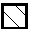
\includegraphics[height=4mm]{bac_shading}}.} 
\lbl{fig:random-subsets}
\end{figure}
% 
Then $X$ and $Y$ are uniformly distributed random variables taking values
in the power sets $\pset(K)$ and $\pset(L)$ respectively, so
% 
\begin{align*}
\Hi(X)  &= \log_2\bigl(2^{\mg{K}}\bigr) = \mg{K}, \\
\Hi(Y)  &= \log_2\bigl(2^{\mg{L}}\bigr) = \mg{L}.
\end{align*}
% 
The random variable $(X, Y)$, which takes values in $\pset(K) \times
\pset(L)$, is uniformly distributed on the set of pairs
\[
\bigl\{ 
(A, B) \in \pset(K) \times \pset(L) 
\such 
A = C \cap K \text{ and } B = C \cap L
\text{ for some } C \sub K \cup L
\bigr\}.
\]
Such pairs are in one-to-one correspondence with subsets of $K \cup L$, so
the entropy of $(X, Y)$ is equal to the entropy of the uniform distribution
on $\pset(K \cup L)$.  Hence
\[
\Hi(X, Y)
=
\log_2 \bigl( 2^{\mg{K \cup L}} \bigr)
=
\mg{K \cup L}.
\]
Then by definition of conditional entropy and mutual information,
% 
\begin{align*}
\condenti{X}{Y} &
=
\mg{K \cup L} - \mg{L} 
= 
\mg{K \without L},     \\
\condenti{Y}{X} &
=
\mg{K \cup L} - \mg{K} 
= 
\mg{L \without K},     \\
I^{\binsym}(X; Y)       &
=
\mg{K} + \mg{L} - \mg{K \cup L} 
=
\mg{K \cap L}.
\end{align*}
% 
So, this example realizes the various entropies shown in the Venn diagram
of Figure~\ref{fig:venn-info} as actual cardinalities.%
%
\index{cardinality}
\end{example}


\subsection*{Extremal cases}

We finish this introduction to joint entropy, conditional entropy and
mutual information by finding their maximal and minimal values in terms of
ordinary entropy.  Here is the central fact.

\begin{lemma}
\lbl{lemma:mut-lb}
$I(X; Y) \geq 0$, with equality if and only if $X$ and $Y$ are independent.
\end{lemma}

\begin{proof}
Lemma~\ref{lemma:mut-alts}\bref{part:mut-alts-mean-rel} states that
\[
I(X; Y) 
= 
\sum_{y \csuch \Pr(y) > 0} \Pr(y) 
\relEnt{(X \given y)}{X}.
\]
Given $y \in \YY$ such that $\Pr(y) > 0$, Lemma~\ref{lemma:rel-ent-pos-def}
implies that $\relEnt{(X \given y)}{X} \geq 0$, with equality if and only
if $\Pr(x \given y) = \Pr(x)$ for all $x \in \XX$.  Thus, $I(X; Y) \geq 0$,
with equality if and only if $\Pr(x \given y) = \Pr(x)$ for all $x$, $y$
such that $\Pr(y) > 0$.  But this condition is equivalent to $X$ and $Y$
being independent.
\end{proof}

\begin{remark}
Given three random variables $X$, $Y$ and $Z$ with the same sample
space, one can define a threefold%
% 
\index{mutual information!threefold}
% 
mutual information $I(X; Y; Z)$ by the same inclusion-exclusion principle
that has guided us so far:
\begin{multline*}
I(X; Y; Z) 
% \\
=
\bigl( H(X) + H(Y) + H(Z) \bigr) 
-
\bigl( H(X, Y) + H(X, Z) + H(Y, Z) \bigr)
\\+
H(X, Y, Z).
\end{multline*}
But in contrast to the binary case, $I(X; Y; Z)$ is sometimes
negative.  For example, this is the case when all three random variables
take values in $\{0, 1\}$ and $(X, Y, Z)$ is uniformly distributed on the
four triples
\[
(0, 0, 0), \ (0, 1, 1), \ (1, 0, 1), \ (1, 1, 0),
\]
with probability zero on the other four.  For discussion of this and other
multivariate information measures, see Timme et al.~\cite{TAFB}, especially
Section~4.2.
\end{remark}

The following proposition gathers together the various maximal and minimal
values and the conditions under which they are attained.  All the results
are as one would guess from the Venn diagrams of Figure~\ref{fig:venn-info}
and~\ref{fig:venn-special}. 

\begin{propn}
\lbl{propn:pair-bounds}
\begin{enumerate}
\item 
\lbl{part:joint-bounds}
Joint entropy is bounded as follows:
\begin{enumerate}
\item 
$\max\{H(X), H(Y)\} \leq H(X, Y) \leq H(X) + H(Y)$;

\item
$H(X, Y) = \max\{H(X), H(Y)\}$ if and only if $X$ is determined by $Y$ or
  $Y$ is determined by $X$;

\item
$H(X, Y) = H(X) + H(Y)$ if and only if $X$ and $Y$ are independent.
\end{enumerate}

\item
\lbl{part:cond-bounds}
Conditional entropy is bounded as follows:
% 
\begin{enumerate}
\item 
$0 \leq \condent{X}{Y} \leq H(X)$;

\item
$\condent{X}{Y} = 0$ if and only if $X$ is determined by $Y$;

\item
$\condent{X}{Y} = H(X)$ if and only if $X$ and $Y$ are independent.
\end{enumerate}

\item
\lbl{part:mut-bounds}
Mutual information is bounded as follows:
% 
\begin{enumerate}
\item 
$0 \leq I(X; Y) \leq \min \{H(X), H(Y)\}$;

\item
$I(X; Y) = 0$ if and only if $X$ and $Y$ are independent;

\item
$I(X; Y) = \min \{H(X), H(Y)\}$ if and only if $X$ is determined by $Y$ or
  $Y$ is determined by $X$.
\end{enumerate}
\end{enumerate}
\end{propn}

\begin{proof}
We begin with~\bref{part:cond-bounds}, using
Lemma~\ref{lemma:cond-alts}\bref{part:cond-alts-cond}: 
\[
\condent{X}{Y} 
=
\sum_{y \csuch \Pr(y) > 0} \Pr(y) H(X \given y).
\]
For each $y$ such that $\Pr(y) > 0$,
Lemma~\ref{lemma:ent-max-min}\bref{part:ent-min} implies that $H(X \given
y) \geq 0$, with equality if and only if there is some $x$ such that $\Pr(x
\given y) = 1$.  So, $\condent{X}{Y} \geq 0$, with equality if and only if
$X$ is determined by $Y$.  For the upper bound, Lemma~\ref{lemma:mut-lb}
gives 
\[
H(X) - \condent{X}{Y} = I(X; Y) \geq 0,
\]
with equality if and only if $X$ and $Y$ are independent.

For~\bref{part:joint-bounds}, we have
\[
H(X, Y) - H(X) = \condent{Y}{X} \geq 0,
\]
with equality if and only if $Y$ is determined by $X$
(by~\bref{part:cond-bounds}).  Hence $H(X, Y) \geq \max\{H(X), H(Y)\}$, and
if equality holds then $Y$ is determined by $X$ or vice versa.  Conversely,
suppose without loss of generality that $Y$ is determined by $X$.  We
have $H(X, Y) = H(X)$ by Example~\ref{egs:joint}\bref{eg:joint-det}
and $H(Y) \leq H(X)$ by Example~\ref{egs:cond}\bref{eg:cond-det}, so
$H(X, Y) = \max\{H(X), H(Y)\}$, as required.  For the upper bound on $H(X,
Y)$, we have
\[
H(X) + H(Y) - H(X, Y) = I(X; Y) \geq 0
\]
with equality if and only if $X$ and $Y$ are independent, by
Lemma~\ref{lemma:mut-lb}. 

For~\bref{part:mut-bounds}, the lower bound and its equality condition
were proved as Lemma~\ref{lemma:mut-lb}.  The upper bound follows from the
lower bound in~\bref{part:joint-bounds} by subtracting from $H(X) +
H(Y)$:
% 
\begin{align*}
&
\max\{H(X), H(Y)\} \leq H(X, Y)         \\
\iff
&
H(X) + H(Y) - \max\{H(X), H(Y)\} 
\geq H(X) + H(Y) - H(X, Y)      \\
\iff
&
\min\{H(X), H(Y)\} \geq I(X; Y),
\end{align*}
% 
with the same condition for equality as in~\bref{part:joint-bounds}.
\end{proof}

\begin{remark}
\lbl{rmk:ub-coupling} 
Given random variables $X$ and $Y$ taking values in finite sets $\XX$ and
$\YY$ respectively, there is a random variable $X \otimes Y$ taking values
in $\XX \times \YY$, the \demph{independent coupling}%
%
\index{coupling!independent}%
\index{independent!coupling}
%
of $X$ and $Y$, with
distribution
\[
\Pr\bigl( X \otimes Y = (x, y) \bigr)
=
\Pr(X = x) \Pr(Y = y)
\]
($x \in \XX$, $y \in \YY$).  That is, if $X$ has distribution $\p$ and $Y$
has distribution $\vc{r}$ then $X \otimes Y$ has distribution $\p \otimes
\vc{r}$.  Then
\[
H(X \otimes Y) = H(X) + H(Y)
\]
by Corollary~\ref{cor:ent-log}, so the upper bound in
Proposition~\ref{propn:pair-bounds}\bref{part:joint-bounds} is equivalent
to
\[
H(X, Y) \leq H(X \otimes Y).
\]
Another way to state this is as follows.  Take probability distributions
$\p$ on $\XX$ and $\vc{r}$ on $\YY$.  Then among all probability
distributions on $\XX \times \YY$ with marginals $\p$ and $\vc{r}$,
none has greater entropy than $\p \otimes \vc{r}$.

This is a special property of \emph{Shannon} entropy.  It does not hold for
any of the other R\'enyi entropies $H_q$ or $q$-logarithmic entropies $S_q$
except, trivially, when $q = 0$.  Counterexamples are given in
Appendix~\ref{sec:max-cpl}.  There is a substantial literature on the
entropy of couplings; see, for instance, Sason~\cite{Saso},
Kova\v{c}evi\'{c}, Stanojevi\'{c} and \v{S}enk~\cite{KSS}, and references
therein.
\end{remark}


\section{Diversity measures for subcommunities}
\lbl{sec:mm-sub}
\index{subcommunity!diversity measures}
\index{diversity measure!subcommunity}


In the next two sections, we introduce quantities measuring
features of a large community of organisms (a \dmph{metacommunity}) divided
into smaller communities (\demph{subcommunities}\index{subcommunity}), to
answer the ecological questions posed in the introduction to this
chapter.  As before, we use terminology inspired by ecology, even though
the mathematics applies far more generally to any types of object.

We have already discussed several times a special type of metacommunity,
namely, a group of islands%
%
\index{islands!subcommunities@as subcommunities} 
% 
(Examples~\ref{eg:comp-islands}, \ref{eg:div1-chain-islands}, \ref{eg:oil},
etc.).  There, the subcommunities are the islands, the metacommunity is the
union of all of them, and a very strong assumption is made: that no species
are shared between islands. Although this is a useful hypothetical extreme
case, it is not realistic.  In the metacommunities that we are about to
consider, each species may be present in one, many, or all of the
subcommunities, in any proportions.

In ecology, there is established terminology for measures of metacommunity
diversity:
% 
\begin{itemize}
\item 
the \dmph{alpha-diversity}\lbl{p:alpha-ave} is the \underline{a}verage
diversity of the subcommunities (in some sense of `average');

\item
the \dmph{beta-diversity}\lbl{p:beta-bet} is the variation \underline{b}etween
the subcommunities;%
%
\index{partitioning of diversity}%
\index{diversity!partitioning of}

\item
the \dmph{gamma-diversity} is the diversity of the whole metacommunity (the
\underline{g}lobal diversity), ignoring its division into subcommunities.
\end{itemize}
% 
These terms were introduced by the ecologist Robert
Whittaker%
%
\index{Whittaker, Robert} 
%
in an influential paper of 1960 (\cite{WhitVSM}, p.~320).  As Tuomisto%
%
\index{Tuomisto, Hanna}
%
observed in a survey paper on beta-diversity, `Obviously, Whittaker~(1960)
did not have an exact definition of beta diversity in mind' (\cite{Tuom1},
p.~2).  However, a large number of specific proposals have been made for
defining these three quantities mathematically.  Some early work on the
subject may have been inspired by analysis%
%
\index{analysis of variance} 
%
of variance (ANOVA) in statistics, where one seeks to quantify
within-group and between-group variation.  But the broad concepts
of alpha-, beta- and gamma-diversity acquired their own independent
standing long ago.

This section and the next are largely based on a paper of Reeve
et al.~\cite{HPD} that sets
out a comprehensive and non-traditional suite of diversity measures for
metacommunities and their subcommunities.  The system of measures is highly
flexible, incorporating both the parameter $q$ (to allow different
emphasis on rare and common species) and the similarity matrix $Z$ (to
encode the different similarities between species).
% 
Here, we confine ourselves to the very special case where $q = 1$ and
$Z = I$ (thus, ignoring inter-species similarity).  Even so, we will be
able to see some of the power and subtlety of the system.  

We begin by fixing our notation (Figure~\ref{fig:Ppw}).  The metacommunity
consists of a collection of individuals, each of which belongs to exactly
one of $S$ species (numbered as $1, \ldots, S$) and exactly one of $N$
subcommunities (numbered as $1, \ldots, N$).  We write $P_{ij}$\ntn{Pij}
for the proportion or relative abundance of individuals belonging to 
the $i$th species and the $j$th subcommunity.
% 
\begin{figure}
\centering
\vspace*{8mm}
\begin{align*}
\lengths
\begin{picture}(0,0)
\put(19,14){\vector(-1,0){11.5}}
\put(19,14){\vector(1,0){11.5}}
\cell{19}{18}{c}{subcommunities}
% 
\put(-6,1){\vector(0,-1){7}}
\put(-6,1){\vector(0,1){7}}
\cell{-10}{1}{c}{\rotatebox{90}{species}}
\end{picture}
P &
=
\begin{pmatrix}
P_{11}  &\cdots &P_{1N} \\
\vdots  &       &\vdots \\
P_{S1}  &\cdots &P_{SN}
\end{pmatrix}
\hspace*{5mm}
\p      
=
\begin{pmatrix}
p_1     \\
\vdots  \\
p_S     
\end{pmatrix}
\\[3mm]
\vc{w}  &
=
\,
\begin{pmatrix}
\,w_1    &\ \cdots\ &w_N\,
\end{pmatrix}
\end{align*}
\caption{Notation for the relative abundances in a metacommunity.}
\lbl{fig:Ppw}
\end{figure}
% 
Thus, $\sum_{i, j} P_{ij} = 1$.  We adopt the convention that
the index $i$ ranges over the set $\{1, \ldots, S\}$ of species and the
index $j$ ranges over the set $\{1, \ldots, N\}$ of subcommunities.

For each species $i$, write
\[
p_i = \sum_j P_{ij},
\ntn{pi}
\]
which is the relative abundance of species $i$ in the whole metacommunity.
Then $\sum_i p_i = 1$.  For each subcommunity $j$, write
\[
w_j = \sum_i P_{ij},
\ntn{wj}
\]
which is the relative size of subcommunity $j$ in the metacommunity.  Then
$\sum_j w_j = 1$.

In purely mathematical terms, the matrix $P$\ntn{Pmx} defines a probability
distribution on the set $\{1, \ldots, S\} \times \{1, \ldots, N\}$, with
marginal distributions 
\[
\p = (p_1, \ldots, p_S)\ntn{pvec},
\qquad
\vc{w} = (w_1, \ldots, w_N)\ntn{wvec}.  
\]
To translate into the language of random variables, we will consider a
random variable $(X, Y)$ taking values in $\{1, \ldots, S\} \times \{1,
\ldots, N\}$, with distribution $P$.  Then $X$ is a random variable with
values in $\{1, \ldots, S\}$ and distribution $\p$, and $Y$ is a random
variable with values in $\{1, \ldots, N\}$ and distribution $\vc{w}$.
Thus, $X$ is a random species and $Y$ is a random subcommunity.

What are the ecological meanings of the joint entropy, conditional entropy
and mutual information of the random variables $X$ and $Y$?  And what are
the roles of relative and cross entropy?  We have seen that when measuring
diversity, it is more appropriate to use the \emph{exponential} of entropy
than entropy itself (Section~\ref{sec:ent-div}, especially
Example~\ref{eg:plague}).  So it is better to ask: what are the ecological
meanings of the exponentials of relative entropy, mutual information, and
so on?

We now proceed to answer these questions, following throughout the notation and
terminology of Reeve et al.~\cite{HPD}.  

First, consider the two entropies defined for a pair of
distributions on the \emph{same} set: relative and cross entropy.  The
$j$th subcommunity has species distribution
\[
P_{\Pdot j}/w_j
=
\bigl( P_{1j}/w_j, \ldots, P_{Sj}/w_j \bigr),
\ntn{Pdotj}
\]
which is the normalization of the $j$th column $P_{\Pdot j}$ of the matrix
$P$.  (Assume that the $j$th subcommunity is nonempty: $w_j > 0$.)
We write
\[
\ovln{\alpha}_j(P) 
=
D(P_{\Pdot j}/w_j)
=
\exp H(P_{\Pdot j}/w_j)
\ntn{alphabar}
\]
for the diversity of order $1$ of the $j$th subcommunity, and call it the
\demph{subcommunity alpha-diversity}.%
%
\index{subcommunity!alpha-diversity}%
\index{alpha-diversity!subcommunity}
% 
Thus, $\ovln{\alpha}_j(P)$ depends on the $j$th subcommunity only, and is
unaffected by the rest of the metacommunity.  Here $D$ denotes the
Hill number $D_1$ of order $1$ (as in Section~\ref{sec:ent-div}); 
no other value of the parameter $q$ is under consideration.

As well as considering the $j$th subcommunity in isolation, we can compare
its species distribution $P_{\Pdot j}/w_j$ with the species distribution
$\p$ of the whole metacommunity, using the relative entropy
$\relent{P_{\Pdot j}/w_j}{\p}$.  Better, we can use the exponential of
relative entropy, which is a relative%
%
\index{relative diversity}
%  
diversity in the sense of Section~\ref{sec:rel-div}.  Thus, we define the
\demph{subcommunity%
%
\index{beta-diversity!subcommunity}%
\index{subcommunity!beta-diversity}
% 
beta-diversity} $\ovln{\beta}_j(P)$ by
% 
\begin{equation}
\ovln{\beta}_j(P)       
=
\reldiv{P_{\Pdot j}/w_j}{\p}
=
\prod_i \Biggl( \frac{P_{ij}}{p_i w_j} \Biggr)^{P_{ij}/w_j}.
\lbl{eq:betaj-exp}      
\end{equation}
% 
This is the diversity of the species distribution of the $j$th subcommunity
relative to that of the metacommunity.  As established in
Section~\ref{sec:rel-div}, it reflects the unusualness or atypicality of
the subcommunity in the context of the metacommunity as a whole.  For
example, if the subcommunity is exactly representative of the whole
metacommunity then $\ovln{\beta}_j(P)$ takes its minimum possible value, $1$. 

(Reeve et al.\ also defined quantities called $\alpha_j$ and $\beta_j$, not
discussed here.  The bars are used in that work to indicate normalization
by subcommunity size.)

Alternatively, we can compare a subcommunity with the metacommunity using
cross%
%
\index{cross entropy} 
% 
entropy rather than relative entropy.  The exponential
$\crossdiv{P_{\Pdot j}/w_j}{\p}$ of the cross entropy is a cross%
%
\index{cross diversity} 
% 
diversity (again in the sense of Section~\ref{sec:rel-div}), and is called
the \demph{subcommunity%
%
\index{gamma-diversity!subcommunity}%
\index{subcommunity!gamma-diversity}
% 
gamma-diversity},
% 
\begin{align}
\gamma_j(P)     &
=
\crossdiv{P_{\Pdot j}/w_j}{\p}
=
\prod_i \Biggl( \frac{1}{p_i} \Biggr)^{P_{ij}/w_j}.
\lbl{eq:gammaj-exp}
\end{align}
% 
Thus, $\gamma_j(P)$ is the cross diversity of the species distribution of
the $j$th subcommunity with respect to that of the metacommunity.  It is
the average rarity of species in the subcommunity, measuring rarity by the
standards of the metacommunity (and using the geometric mean as our notion
of average).  For example, if the subcommunity is exactly representative of
the metacommunity then $\gamma_j(P)$ is just the diversity of the
metacommunity. 

Other examples of relative diversity and cross diversity were given in
Section~\ref{sec:rel-div}, illustrating the ecological meanings of high or
low values of $\ovln{\beta}_j(P)$ or $\gamma_j(P)$.

Equation~\eqref{eq:rco} (p.~\pageref{eq:rco}) implies that
% 
\begin{equation}
\lbl{eq:abg}
\ovln{\alpha}_j(P) \cdot \ovln{\beta}_j(P) = \gamma_j(P).
\end{equation}
% 
This identity can be understood as follows:
% 
\begin{itemize}
\item
$\ovln{\alpha}_j(P)$ measures how unusual
the average individual is within the subcommunity;

\item
$\ovln{\beta}_j(P)$ measures how unusual the subcommunity is within the
  metacommunity;

\item
$\gamma_j(P)$ measures how unusual the average individual in the
  subcommunity is within the metacommunity.
\end{itemize}
% 
Thus, equation~\eqref{eq:abg} partitions%
%
\index{partitioning of diversity}%
\index{diversity!partitioning of}
% 
the global diversity measure $\gamma_j(P)$ into components measuring
diversity at different levels of resolution.

In the next section, we explain the connection between, on the one hand,
the \emph{subcommunity} alpha-, beta- and gamma-diversities just defined,
and, on the other, what ecologists usually call alpha-, beta- and
gamma-diversity, which are quantities associated with the
\emph{metacommunity}.  We will use the language of random variables.  In
that language, the subcommunity measures that we have just defined are
given by
% 
\begin{align*}
\ovln{\alpha}_j(P)      &
=
\exp\bigl( H(X \given j) \bigr),        \\
\ovln{\beta}_j(P)  &
=
\exp\Bigl( \relEnt{(X \given j)}{X} \Bigr),     \\
\gamma_j(P)        &
=
\exp\Bigl( \crossEnt{(X \given j)}{X} \Bigr),
\end{align*}
% 
since the distribution of the conditional random variable $X \given j$ is
the species distribution $P_{\Pdot j}/w_j$ in the $j$th subcommunity.


\section{Diversity measures for metacommunities}
\lbl{sec:mm-meta}
\index{diversity measure!metacommunity}
\index{metacommunity!diversity measures}


In the last section, the alpha-, beta- and gamma-diversities of the $j$th
subcommunity were defined by comparing two random variables taking values
in the set of species: $X \given j$, which is the species of an individual
chosen at random from the $j$th subcommunity, and $X$, which is the species
of an individual chosen at random from the whole metacommunity.

In this section, we derive measures of the metacommunity by comparing two
random variables taking values in different sets: the species $X$ and the
subcommunity $Y$ of an individual chosen at random from the metacommunity.
Specifically, we consider the exponentials of their joint entropy,
conditional entropies, and mutual information.

Figure~\ref{fig:mc-measures}\hardref{(a)} summarizes the situation, with
the previous Venn diagram for entropies (Figure~\ref{fig:venn-info})
reproduced in~\hardref{(b)} for reference.  The notation in~\hardref{(a)}
is again taken from Reeve et al.~\cite{HPD}, and each term is now explained in
turn.  Tables~\ref{table:mcm-desc} and~\ref{table:mcm-range} give 
summaries.

\begin{figure}
\centering
\lengths
\begin{picture}(54,35)(0,-5)
\cell{27}{17}{c}{\includegraphics[height=26\unitlength]{venn_shadedm}}
\cell{7}{25}{c}{$G$}
\cell{49.5}{25}{c}{$D(\vc{w})$}
\cell{14}{17}{c}{$\ovln{A}$}
\cell{27}{17}{c}{$\ovln{B}$}
\cell{40}{16.5}{c}{$R$}
\cell{27}{1}{b}{$A$}
\cell{27}{-5}{b}{(a)}
\end{picture}%
\hspace*{12mm}%
\begin{picture}(54,35)(0,-5)
\cell{27}{17}{c}{\includegraphics[height=26\unitlength]{venn_shadedm}}
\cell{5}{25}{c}{$H(X)$}
\cell{49}{25}{c}{$H(Y)$}
\cell{14}{17}{c}{$\condent{X}{Y}$}
\cell{27}{17}{c}{$I(X; Y)$}
\cell{40}{17}{c}{$\condent{Y}{X}$}
\cell{27}{0.5}{b}{$H(X, Y)$}
\cell{27}{-5}{b}{(b)}
\end{picture}
\caption{The metacommunity gamma-diversities, shown in~\hardref{(a)}, are
  the exponentials of the entropies shown in~\hardref{(b)}.  For instance,
  $\ovln{A}(P) = \exp \condent{X}{Y}$.}  
\lbl{fig:mc-measures}
\end{figure}

\begin{table}
\centering
\begin{tabular}{lll@{\hspace{2.8mm}}l}
\hline
Quantity        &
Name            &
Formula &
Description     \\
\hline
$\exp H(X)$     &
$G(P)$          &
$\displaystyle\prod_i \Biggl( \frac{1}{p_i} \Biggr)^{p_i\vphantom{X^X_X}}$&
Effective no.\ of species in metacommunity,   \\[-1.9ex]
&
&
&
ignoring division into subcommunities   \\[1.7ex]
$\exp H(Y)$     &
$D(\vc{w})$     &
$\displaystyle\prod_j \Biggl( \frac{1}{w_j} \Biggr)^{w_j}$     &
Effective no.\ of subcommunities in meta-\\[-1.9ex]
&
&
&
community, ignoring division into species          \\[1.7ex]
$\exp H(X, Y)$  &
$A(P)$     &
$\displaystyle\prod_{i, j} \Biggl( \frac{1}{P_{ij}} \Biggr)^{P_{ij}}$  &
Effective no.\ of (species, subcommunity)       \\[-1.9ex]
&
&
&
pairs   \\[1.7ex]
$\exp \condent{X}{Y}$   &
$\ovln{A}(P)$      &
$\displaystyle\prod_{i, j} \Biggl( \frac{w_j}{P_{ij}} \Biggr)^{P_{ij}}$ &
Average effective no.\ of species per    \\[-1.9ex]
&
&
&
subcommunity        \\[1.7ex]
$\exp \condent{Y}{X}$   &
$R(P)$     &
$\displaystyle\prod_{i, j} \Biggl( \frac{p_i}{P_{ij}} \Biggr)^{P_{ij}}$ &
% Metacommunity redundancy    \\[1.7ex]
Redundancy of subcommunities \\[1.7ex]
$\exp I(X; Y)$  &
$\ovln{B}(P)$      &
$\displaystyle\prod_{i, j} \Biggl( \frac{P_{ij}}{p_i w_j} \Biggr)^{P_{ij}}$&
Effective no.\ of isolated subcommunities     \\
\hline
\end{tabular}
\index{effective number!species@of species}%
\index{effective number!subcommunities@of subcommunities}%
\caption{Formulas for and descriptions of the metacommunity diversity
  measures.  The first product is over the support of $\p$, the second is
  over the support of $\vc{w}$, and the others are over the support of
  $P$.}
\lbl{table:mcm-desc}
\end{table}

\begin{table}
\centering
\begin{tabular}{|l|l|l|l|}
\hline
Name            &
Range           &
Minimized when  &
Maximized when  \\
\hline
$G(P)$          &
$[1, S]\vphantom{X^{X^X}}$        &
Only one species in        &
Species in metacommunity    \\
&
&
metacommunity       &
are balanced        \\[1ex]
$D(\vc{w})$     &
$[1, N]$        &
Only one subcommunity in  &
Subcommunities are same \\
&
&
metacommunity        &
size    \\[1ex]
$A(P)$          &
$[1, SN]$       &
Only one species and one        &
Subcommunities are same     \\
&
&
subcommunity in&
size and all balanced        \\
&
&
metacommunity&
\\[1ex]
$\ovln{A}(P)$   &
$[1, S]$        &
Each subcommunity contains      &
Each subcommunity is  \\
&
&
only one species        &
balanced        \\[1ex]
$R(P)$          &
$[1, N]$        &
Subcommunities share no         &
Subcommunities have same    \\
&
&
species &
size and composition    \\[1ex]
$\ovln{B}(P)$   &
$[1, N]$        &
Subcommunities have same        &
Subcommunities have same   \\
&
&
composition     &
size and share no species    \\
\hline
\end{tabular}
\caption{Minimum and maximum values of the metacommunity diversity
  measures.  The bounds shown depend only on $S$ and $N$; tighter bounds
%   relating the measures to one another 
  are given in the text.
  \demph{Balanced}\index{balanced} means that all species have equal
  abundance.}  
\lbl{table:mcm-range}
\end{table}


\subsection*{Metacommunity gamma-diversity}

First consider the random variable $X$ for species.  The exponential of its
Shannon entropy $H(X)$ is 
\[
D(\p)
=
\prod_{i \in \supp(\p)} \Biggl( \frac{1}{p_i} \Biggr)^{p_i}.
\]
This is simply the diversity of order $1$ of the species distribution $\p$
of the whole metacommunity, ignoring its division into subcommunities.
(Throughout this section, all diversities are of order~$1$.)  We write
$G(P)\ntn{Gdiv} = D(\p)$ and call it the \demph{metacommunity
  gamma-diversity}.%
%
\index{gamma-diversity!metacommunity}%
\index{metacommunity!gamma-diversity}

The metacommunity gamma-diversity $G(P)$ is related to the subcommunity
gamma-diversities $\gamma_1(P), \ldots, \gamma_N(P)$ as follows:
% 
\begin{align}
G(P)    &
=
\prod_{i, j \csuch i \in \supp(\p)}
\Biggl( \frac{1}{p_i} \Biggr)^{P_{ij}}  
\nonumber       \\
&
=
\prod_j \gamma_j(P)^{w_j}  
\nonumber       \\
&
=
M_0 \Bigl( \vc{w}, \bigl(\gamma_1(P), \ldots, \gamma_N(P)\bigr) \Bigr).
\lbl{eq:G-mean}
\end{align}
% 
Here we have used the definition of $p_i$ as $\sum_j P_{ij}$ and the
formula~\eqref{eq:gammaj-exp} for $\gamma_j(P)$.  So, the metacommunity
gamma-diversity $G(P)$ is the geometric mean of the subcommunity
gamma-diversities $\gamma_j(P)$, weighted by the sizes of the
subcommunities. 

In this sense, the subcommunity gamma-diversity $\gamma_j(P)$ is the mean
contribution~\lbl{p:gamma-contrib} per individual of the $j$th subcommunity
to the metacommunity diversity.

The metacommunity gamma-diversity is constrained by the bounds
\[
1 \leq G(P) \leq S,
\]
by Lemma~\ref{lemma:div1-max-min}.  It attains the lower bound $G(P) = 1$
when the metacommunity consists of a single species, and the upper bound
$G(P) = S$ when all $S$ species have equal abundance in the metacommunity
(regardless of how they are distributed across the subcommunities).

Now consider the random variable $Y$ for subcommunities. The exponential of
$H(Y)$ is
\[
D(\vc{w}) 
=
\prod_{j \in \supp(\vc{w})} \Biggl( \frac{1}{w_j} \Biggr)^{w_j}.
\]
It measures how evenly the population is distributed across the
subcommunities (regardless of how it is distributed across species).  It is
bounded by
\[
1 \leq D(\vc{w}) \leq N
\]
(by Lemma~\ref{lemma:div1-max-min} again), with $D(\vc{w}) = 1$ when the
metacommunity contains only one nonempty subcommunity and $D(\vc{w}) =
N$ when the populations of the $N$ subcommunities are of equal size.  


\subsection*{Metacommunity alpha-diversities}

The joint%
%
\index{joint entropy}
% 
entropy $H(X, Y)$ has exponential
\[
D(P)
=
\prod_{(i, j) \in \supp(P)} 
\Biggl( \frac{1}{P_{ij}} \Biggr)^{P_{ij}}.
\]
Here we are treating the $S \times N$ matrix $P$ as a probability
distribution on the set $\{1, \ldots, S\} \times \{1, \ldots, N\}$.  So,
$D(P)$ is the effective number of (species, subcommunity) pairs, in the
sense of Section~\ref{sec:ent-div}.  It is the species
diversity that the metacommunity would have if individuals in different
subcommunities were decreed to be of different species (as in the island%
%
\index{islands!subcommunities@as subcommunities}
% 
scenario).  We write $A(P)\ntn{Adiv} = D(P)$ and call it the \demph{raw
  metacommunity alpha-diversity}.% 
% 
\index{alpha-diversity!raw metacommunity}%
\index{metacommunity!alpha-diversity, raw}

Since $A(P)$ measures diversity as if no species were shared between
subcommunities, it overestimates the true diversity.  Indeed, taking
exponentials in the inequalities
\[
H(X) \leq H(X, Y) \leq H(X) + H(Y)
\]
of Proposition~\ref{propn:pair-bounds}\bref{part:joint-bounds} gives
% 
\begin{equation}
\lbl{eq:A-bounds}
G(P) \leq A(P) \leq D(\vc{w}) G(P).
\end{equation}
% 
The upper bound states that the factor of overestimation is at most
$D(\vc{w})$, the effective number of subcommunities. 

The minimum value $A(P) = G(P)$ occurs when $H(X, Y) = H(X)$, which by
Proposition~\ref{propn:pair-bounds}\bref{part:cond-bounds} means that $Y$
is determined by $X$: the subcommunity is determined by the species.  So,
$A(P) = G(P)$ when no species are shared between subcommunities.  

The maximum value $A(P) = D(\vc{w})G(P)$ occurs when $H(X, Y) = H(X) +
H(Y)$.  By Proposition~\ref{propn:pair-bounds}\bref{part:joint-bounds},
this is true just when $X$ and $Y$ are independent.  Equivalently, $A(P)$
attains its maximum when the metacommunity is \lbl{p:wm}\dmph{well-mixed},
meaning that each of the subcommunity species distributions $P_{\Pdot
  j}/w_j$ is equal to the metacommunity species distribution $\p$.

In summary: $A(P)$ does not overestimate $G(P)$ at all when the
subcommunities share no species, whereas the overestimation is most
pronounced when all of the subcommunities have identical composition.

Since $1 \leq G(P) \leq S$ and $1 \leq D(\vc{w}) \leq N$, the
inequalities~\eqref{eq:A-bounds} imply the cruder bounds
\[
1 \leq A(P) \leq SN.  
\]
This conforms with the interpretation of $A(P)$ as the effective number
of (species, subcommunity) pairs.  The minimum $A(P) = 1$ is attained when
there is only one species present and only one nonempty subcommunity.  The
maximum $A(P) = SN$ is attained when the metacommunity is well-mixed and the
subcommunities all have the same size.  

Next consider conditional%
%
\index{conditional entropy}
%  
entropy.  By Lemma~\ref{lemma:cond-alts}\bref{part:cond-alts-exp}, the
conditional entropy $\condent{X}{Y}$ is given by
\[
\condent{X}{Y}
=
\sum_{i, j \csuch \Pr(i, j) > 0} 
\Pr(i, j) \log \frac{\Pr(j)}{\Pr(i, j)}.
\]
The \demph{normalized%
%
\index{alpha-diversity!normalized metacommunity}%
\index{metacommunity!alpha-diversity, normalized}
%
metacommunity alpha-diversity} $\ovln{A}(P)$ is its
exponential: 
% 
\begin{equation}
\lbl{eq:Abar-defn}
\ovln{A}(P) 
=
\exp\condent{X}{Y}
=
\prod_{i, j \csuch P_{ij} > 0} 
\Biggl( \frac{w_j}{P_{ij}} \Biggr)^{P_{ij}}.
\end{equation}
% 
To understand $\ovln{A}$, we use one of the other formulas for conditional
entropy:
% 
\begin{equation}
\lbl{eq:Abar-cond}
\condent{X}{Y}
=
\sum_{j \csuch \Pr(j) > 0} \Pr(j) H(X \given j)
\end{equation}
% 
(Lemma~\ref{lemma:cond-alts}\bref{part:cond-alts-cond}).  The random
variable $X \given j$ is the species of a random individual from the $j$th
subcommunity, so taking exponentials throughout
equation~\eqref{eq:Abar-cond} gives
% 
\begin{align}
\ovln{A}(P)        &
=
\prod_{j \csuch w_j > 0} \ovln{\alpha}_j(P)^{w_j}  
\nonumber       \\
&
=
M_0 \Bigl( 
\vc{w}, \bigl(\ovln{\alpha}_1(P), \ldots, \ovln{\alpha}_N(P)\bigr) 
\Bigr).
\lbl{eq:A-mean}
\end{align}
% 
Hence $\ovln{A}(P)$ is the geometric mean of the individual subcommunity
diversities $\ovln{\alpha}_j(P)$, weighted by their sizes.  It is therefore
an alpha-diversity in the traditional sense (Remark~\ref{rmk:abg-rel} and
p.~\pageref{p:alpha-ave}). 

To find the maximum and minimum values of $\ovln{A}$, we take exponentials
throughout the inequalities
\[
0 \leq \condent{X}{Y} \leq H(X)
\]
(Proposition~\ref{propn:pair-bounds}\bref{part:cond-bounds}).  This gives
% 
\begin{equation}
\lbl{eq:Abar-bounds}
1 \leq \ovln{A}(P) \leq G(P),
\end{equation}
% 
with $\ovln{A}(P) = 1$ when each subcommunity contains at most one species
and $\ovln{A}(P) = G(P)$ when the metacommunity is well-mixed.  Since $G(P)
\leq S$, we also have the cruder bounds
\[
1 \leq \ovln{A}(P) \leq S,
\]
with $\ovln{A}(P) = S$ when each subcommunity contains all $S$ species in
equal proportions.

The raw%
%
\index{alpha-diversity!raw metacommunity}%
\index{metacommunity!alpha-diversity, raw}
% 
and normalized% 
%
\index{alpha-diversity!normalized metacommunity}%
\index{metacommunity!alpha-diversity, normalized}
% 
metacommunity alpha-diversities, $A(P)$ and $\ovln{A}(P)$, are linked by
the equation
% 
\begin{equation}
\lbl{eq:AAw}
\ovln{A}(P) = A(P)/D(\vc{w}),
\end{equation}
% 
which is the exponential of the definition
\[
\condent{X}{Y} = H(X, Y) - H(Y)
\]
of conditional entropy. 

\begin{examples}
\lbl{egs:mc-A}
Here we take the four running examples of Section~\ref{sec:mm-info} and
translate them into ecological terms.  The results below follow immediately
from those examples, and are summarized in the first few rows of
Table~\ref{table:mm-egs}.

\begin{table}
\centering
\begin{tabular}{llllll}
\hline 
% Quantity        &Name   &
% \bref{eg:mc-A-ind} Well-mixed &
% \bref{eg:mc-A-one} Only one   &
% \bref{eg:mc-A-equal} Subcomms &
% \bref{eg:mc-A-det} Isolated   \\
Quantity        &Name   &
\bref{eg:mc-A-ind}      &
\bref{eg:mc-A-one}      &
\bref{eg:mc-A-equal}    &
\bref{eg:mc-A-det}      \\
        &       &
Well-mixed      &
Only one        &
Subcomms        &
Isolated        \\
                &       &
% \phantom{\bref{eg:mc-A-ind}} 
metacomm   &
% \phantom{\bref{eg:mc-A-one}} 
subcomm    &
% \phantom{\bref{eg:mc-A-equal}} 
are species     &
% \ \ 
% \phantom{\bref{eg:mc-A-det}} 
subcomms  \\[0ex]
\hline
$\exp H(X)\vphantom{X^{X^X}}$     &
$G(P)$          &
$D(\p)$         &
$D(\p)$         &
$D(\p)$         &
$D(\p)$         \\[1ex]
$\exp H(Y)$     &
$D(\vc{w})$     &
$D(\vc{w})$     &
$1$             &
$D(\p)$         &
$D(\vc{w})$     \\[1ex]
$\exp H(X, Y)$  &
$A(P)$          &
$D(\p)D(\vc{w})$&
$D(\p)$         &
$D(\p)$         &
$D(\vc{w})\ovln{A}(P)$\\[1ex]
$\exp\condent{X}{Y}$&
$\ovln{A}(P)$   &
$D(\p)$         &
$D(\p)$         &
$1$             &
$\ovln{A}(P)$   \\[1ex]
$\exp\condent{Y}{X}$&
$R(P)$          &
$D(\vc{w})$     &
$1$             &
$1$             &
$1$             \\[1ex]
$\exp I(X; Y)$  &
$\ovln{B}(P)$   &
$1$             &
$1$             &
$D(\p)$         &
$D(\vc{w})$     \\
\hline
\end{tabular}
\caption{Summary of Examples~\ref{egs:mc-A} and~\ref{egs:mc-B}.}
\lbl{table:mm-egs}
\end{table}

\begin{enumerate}
\item
\lbl{eg:mc-A-ind}
Suppose that the metacommunity is well-mixed.
Then $P = \p \otimes \vc{w}$ and $A(P) = D(P) = D(\p)D(\vc{w})$.  Each
subcommunity has the same species composition as the metacommunity, so the
mean subcommunity diversity $\ovln{A}(P)$ is the same as the metacommunity
diversity $G(P)$.  

\item
\lbl{eg:mc-A-one}
Suppose that the metacommunity consists of a single subcommunity.  Then $N
= 1$, $\vc{w} = (1)$, and $P = \p$.  The effective number $A(P)$ of
(species, subcommunity) pairs is just the effective number $D(\p)$ of
species, and since there is only one subcommunity, the average subcommunity
diversity $\ovln{A}(P)$ is also $D(\p)$.

\item
\lbl{eg:mc-A-equal}
Suppose that the subcommunities are exactly the species.  Thus, $N = S$,
$\vc{w} = \p$, and $P$ is the diagonal matrix with entries $p_1, \ldots,
p_S$.  The effective number $A(P)$ of (species, subcommunity) pairs is again
just $D(\p)$, but since each subcommunity has a diversity of $1$, the
average subcommunity diversity $\ovln{A}(P)$ is now $1$.  

\item
\lbl{eg:mc-A-det}
Finally, suppose that all subcommunities are isolated (share no species).
Nothing special can be said about $\ovln{A}(P)$, the mean subcommunity
diversity, since it is unaffected by the degree of overlap of species
between subcommunities.  As always, $A(P) = D(\vc{w})\ovln{A}(P)$.
\end{enumerate}
\end{examples}


\subsection*{The redundancy of a metacommunity}

We have already considered one conditional%
%
\index{conditional entropy}
% 
entropy, $\condent{X}{Y}$.  The other,
\[
\condent{Y}{X}
=
\sum_{i, j \csuch \Pr(i, j) > 0} 
\Pr(i, j) \log \frac{\Pr(i)}{\Pr(i, j)},
\]
has exponential
% 
\begin{equation}
\lbl{eq:R-defn}
R(P) = 
\prod_{i, j \csuch P_{ij} > 0} 
\Biggl( \frac{p_i}{P_{ij}} \Biggr)^{P_{ij}}.
\end{equation}
% 
This is the \dmph{redundancy} of the metacommunity.  The word is meant in
the following sense: if some subcommunities were to be destroyed,%
%
\index{subcommunity!loss}
%  
how much of the diversity in the metacommunity would be preserved?  High
redundancy means that there is enough repetition of species across
subcommunities that loss of some subcommunities would probably not
cause great loss of diversity.

We now justify this interpretation.  For each species $i$, consider
the relative abundances $P_{i1}, \ldots, P_{iN}$ of that species within the
$N$ subcommunities, and normalize to obtain a probability distribution
\[
P_{i\,\Pdot}/p_i
=
(P_{i1}/p_i, \ldots, P_{iN}/p_i)
\]
on the set $\{1, \ldots, N\}$ of subcommunities.  (We assume in this
explanation that $p_i > 0$.)  Then $D(P_{i\,\Pdot}/p_i)$ measures the
extent to which the $i$th species is spread evenly across the
subcommunities; for instance, it takes its maximum value $N$ when there is
the same amount of species $i$ in every subcommunity.  This is the
`redundancy' of the $i$th species.  

To obtain a measure of the redundancy of the whole metacommunity, we take
the geometric mean
% 
\begin{equation}
\lbl{eq:R-mean}
\prod_{i \in \supp(\p)} D(P_{i\,\Pdot}/p_i)^{p_i}
\end{equation}
% 
of the redundancies of the species, weighted by their relative abundances.
But this is exactly $R(P)$, since, using
Lemma~\ref{lemma:cond-alts}\bref{part:cond-alts-cond}, 
% 
\begin{align*}
\prod_{i \in \supp(\p)} D(P_{i\,\Pdot}/p_i)^{p_i}       &
=
\exp \Biggl( \sum_{i \in \supp(\p)} p_i H(P_{i\,\Pdot}/p_i) \Biggr) \\
&
=
\exp \Biggl( \sum_{i \csuch \Pr(i) > 0} \Pr(i) \condent{Y}{i} \Biggr)\\
&
=
\exp \condent{Y}{X}     \\
&
=
R(P).
\end{align*}
% 
In conclusion, $R(P)$ is the average species redundancy~\eqref{eq:R-mean}:
the effective number of subcommunities across which a typical species is
spread.

A different way to understand redundancy is through the equation
% 
\begin{equation}
\lbl{eq:GAR}
R = A/G,
\end{equation}
% 
which is the exponential of the definition 
\[
\condent{Y}{X} = H(X, Y) - H(X)
\]
of conditional entropy.  The gamma-diversity $G(P)$ is the effective number
of species in the metacommunity, whereas $A(P)$ is the effective number of
species if we pretend that individuals in different subcommunities are
always of different species.  The amount by which $A(P)$ overestimates
$G(P)$ reflects the extent to which species are, in reality, shared across
subcommunities: thus, it measures redundancy.  

Bounds on the redundancy can be obtained by dividing
inequalities~\eqref{eq:A-bounds} by $G(P)$.  This gives
\[
1 \leq R(P) \leq D(\vc{w}),
\]
with the same extremal cases as for~\eqref{eq:A-bounds}: redundancy takes
its minimum value of $1$ when no species are shared between
subcommunities, and its maximum value of $D(\vc{w})$ when the species
distributions in the subcommunities are all the same.  It follows that
\[
1 \leq R(P) \leq N,
\]
with $R(P) = N$ when the subcommunities have not only the same composition,
but also the same size.  


\subsection*{Metacommunity beta-diversity}

Finally, consider the mutual%
% 
\index{mutual information} 
% 
information $I(X; Y)$.  By
Lemma~\ref{lemma:mut-alts}\bref{part:mut-alts-exp}, its exponential
$\ovln{B}(P)$ is given by
\[
\ovln{B}(P)
=
\prod_{i, j \csuch P_{ij} > 0}
\Biggl( \frac{P_{ij}}{p_i w_j} \Biggr)^{P_{ij}}.
\ntn{Bbardiv}
\]
This is the \demph{metacommunity%
%
\index{beta-diversity!metacommunity}%
\index{metacommunity!beta-diversity}
% 
beta-diversity}.  (In Reeve et al.~\cite{HPD}, it is called the
`normalized' beta-diversity, and there is also a `raw' beta-diversity
$B(P)$, not treated here.)  By the discussion of mutual information in
Section~\ref{sec:mm-info}, $\ovln{B}(P)$ can be understood as the
exponential of the amount of information that knowledge of an individual's
species gives us about its subcommunity~-- or equivalently, vice versa.

Loosely, then, $\ovln{B}(P)$ measures the alignment between subcommunity
structure and species structure.  It is a beta-diversity in the traditional
sense of Remark~\ref{rmk:abg-rel} and p.~\pageref{p:beta-bet}.

By Proposition~\ref{propn:pair-bounds}\bref{part:mut-bounds} on mutual
information,
% 
\begin{equation}
\lbl{eq:Bbar-bounds}
1 \leq \ovln{B}(P) \leq \min \{G(P), D(\vc{w})\}.  
\end{equation}
% 
The minimum $\ovln{B}(P) = 1$ is attained when $X$ and $Y$ are independent,
that is, the metacommunity is well-mixed.  In that case, knowing an
individual's species does not help us to guess its subcommunity,
nor vice versa.  
% 
By Proposition~\ref{propn:pair-bounds}\bref{part:mut-bounds}, there are two
cases in which the maximum is attained.  One is where $X$ is determined by
$Y$, that is, there is at most one species in each subcommunity.  Then by
Example~\ref{egs:cond}\bref{eg:cond-det},
% 
% \begin{equation}
% \lbl{eq:Bbar-loose-bounds}
\[
\ovln{B}(P) = G(P) \leq D(\vc{w}).
\]
% \end{equation}
% 
In this case, knowing the subcommunity to which an individual belongs
enables us to infer its species with certainty.  The other case in which
the maximum is attained is where $Y$ is determined by $X$, that is, the
subcommunities are isolated.  Then
\[
\ovln{B}(P) = D(\vc{w}) \leq G(P)
\]
by Example~\ref{egs:cond}\bref{eg:cond-det} again, and knowing an
individual's species enables us to infer its subcommunity with certainty.

We can also interpret $\ovln{B}$ as the effective%
%
\index{effective number!subcommunities@of subcommunities}%
\index{subcommunity!effective number of isolated}
% 
number of isolated subcommunities.  Indeed, since $1 \leq D(\vc{w}) \leq
N$, the inequalities~\eqref{eq:Bbar-bounds} imply that
% 
\begin{equation}
\lbl{eq:Bbar-crude}
1 \leq \ovln{B}(P) \leq N.
\end{equation}
% 
The maximum $\ovln{B}(P) = N$ occurs when the $N$ subcommunities are
isolated and of equal size.  We will see in
Proposition~\ref{propn:mc-chain} and Corollary~\ref{cor:mc-rep} that
$\ovln{B}$ satisfies a chain rule and a replication principle, supporting
the effective number interpretation.

For yet another viewpoint on $\ovln{B}$, recall from
equations~\eqref{eq:mut-alt} that
\[
\condent{X}{Y} + I(X; Y) = H(X).
\]
Taking exponentials throughout gives
% 
\begin{equation}
\lbl{eq:ABG}
\ovln{A} \, \ovln{B} = G,
\end{equation}
% 
that is,
\[
\text{alpha-diversity} \times \text{beta-diversity}
=
\text{gamma-diversity}.
\]
This equation partitions%
%  
\index{partitioning of diversity}%
\index{diversity!partitioning of}
% 
the diversity of the metacommunity (gamma) into two components: the average
diversity within subcommunities (alpha) and the variation between
subcommunities (beta).  The general principle has a long history, going
back to the foundational work of Whittaker%
%
\index{Whittaker, Robert} 
% 
(p.~321 of~\cite{WhitVSM} and p.~232 of~\cite{WhitEMS}).

From equations~\eqref{eq:ABG}, \eqref{eq:AAw} and~\eqref{eq:GAR}, it
follows that 
\[
\ovln{B}(P)
=
\frac{G(P)}{\ovln{A}(P)}
=
\frac{G(P)D(\vc{w})}{A(P)} 
=
\frac{D(\vc{w})}{R(P)}, 
\]
giving
\[
\ovln{B}(P) = \frac{D(\vc{w})}{R(P)}.
\]
So when the subcommunity sizes $\vc{w}$ are fixed, the effective number
$\ovln{B}(P)$ of isolated subcommunities is inversely proportional to the
redundancy $R(P)$.  This is reasonable: $R(P)$ measures overlap of species
between subcommunities, whereas $\ovln{B}(P)$ measures how disjoint the 
subcommunities are.

(Matters are more subtle outside the case $q = 1$, $Z = I$ to which we have
confined ourselves.  When $q \neq 1$ in the work of Reeve et al., the
dependency between $\ovln{B}$ and $R$ breaks down, in the strong sense that
the two quantities no longer determine one another; they convey
different information.)

\begin{examples}
\lbl{egs:mc-B}
We return to the four scenarios of Examples~\ref{egs:mc-A}, finding the
redundancy\index{redundancy} $R(P)$ and metacommunity beta-diversity
$\ovln{B}(P)$.  The results are summarized in Table~\ref{table:mm-egs}.
% 
\begin{enumerate}
\item
\lbl{eg:mc-B-ind}
A well-mixed metacommunity is maximally redundant ($R(P) = D(\vc{w})$),
since all subcommunities are identical.  For the same reason, the effective
number $\ovln{B}(P)$ of isolated subcommunities is just $1$.

\item
\lbl{eg:mc-B-one}
If the metacommunity consists of a single subcommunity ($N = 1$) then the
redundancy $R(P)$ and effective number $\ovln{B}(P)$ of isolated
subcommunities both take their minimum values of $1$.  

\item
\lbl{eg:mc-B-equal}
Suppose that the subcommunities are exactly the species.  Then 
the metacommunity is minimally redundant ($R(P) = 1$), reflecting the fact
that each species is present in just one subcommunity: losing any of the
subcommunities means losing a species.  And since subcommunities are
species, the effective number $\ovln{B}(P)$ of isolated subcommunities is the
effective number $D(\p)$ of species.  

\item
\lbl{eg:mc-B-det}
More generally, suppose that all subcommunities are isolated.  The
redundancy is minimal ($R(P) = 1$), since no species is repeated across
subcommunities.  The effective number $\ovln{B}(P)$ of isolated
subcommunities is simply the diversity $D(\vc{w})$ of the subcommunity
distribution $\vc{w}$, which is reasonable since, in fact, the
subcommunities \emph{are} isolated.
\end{enumerate}
\end{examples}

Just as the metacommunity gamma-diversity $G(P)$ is the geometric mean of
the subcommunity gamma-diversities $\gamma_j(P)$, and just as the
metacommunity alpha-diversity $\ovln{A}(P)$ is the geometric mean of the
subcommunity alpha-diversities $\ovln{\alpha}_j(P)$, the metacommunity
beta-diversity $\ovln{B}(P)$ is the geometric mean of the subcommunity
beta-diversities $\ovln{\beta}_j(P)$.  Indeed, recall from
Lemma~\ref{lemma:mut-alts}\bref{part:mut-alts-mean-rel} that
\[
I(X; Y)
=
\sum_{j \csuch \Pr(j) > 0} \Pr(j) \relEnt{(X \given j)}{X}.
\]
Taking exponentials throughout gives
% 
\begin{align}
\ovln{B}(P)        &
=
\prod_{j \csuch w_j > 0} \ovln{\beta}_j(P)^{w_j}   
\nonumber       \\
&
=
M_0 \Bigl( \vc{w}, \bigl(\ovln{\beta}_1(P), \ldots, \ovln{\beta}_N(P)\bigr) 
\Bigr),
\lbl{eq:B-mean}
\end{align}
% 
as claimed.

We have seen that $\ovln{\beta}_j(P)$ measures how unusual the $j$th
subcommunity is in the context of the metacommunity.  Taking the geometric
mean over all subcommunities gives $\ovln{B}(P)$, which is therefore an
overall measure of the atypicality or isolation of the subcommunities
within the metacommunity.

Further connections between beta-diversity and information-theoretic
quantities are described in the first appendix of the paper~\cite{HPD} of
Reeve et al.


\section{Properties of the metacommunity measures}
\lbl{sec:mm-props}
\index{metacommunity!diversity measures}
\index{diversity measure!metacommunity}


In this chapter so far, we have introduced a system of measures of the
diversity and structure of a metacommunity, and explained their behaviour
in a variety of hypothetical examples.  But just as a measure of the
diversity of a \emph{single} community should not be accepted or used until
it can be shown to behave logically (Section~\ref{sec:ent-div}), the
metacommunity measures should also be required to have sensible logical and
algebraic properties.  Here we show that they do.


\subsection*{Independence}

We begin by showing that the alpha-diversity $\ovln{A}$ and beta-diversity
$\ovln{B}$ are independent~-- not in the sense of probability theory, but in
the sense of \emph{certain} knowledge.  An informal example illustrates the
idea.  Assume for simplicity that every person in the world is
either dark-haired%
%
\index{hair colour} 
% 
or fair-haired, and either brown-eyed%
%
\index{eye colour}
% 
or blue-eyed.  These two variables, hair colour and eye colour, are not
independent in the probabilistic sense: people with dark hair are more
likely to have dark eyes.  However, they are independent in a weaker sense:
knowing an individual's hair colour gives no \emph{certain} knowledge of
their eye colour, nor vice versa.  All four combinations occur.

The formal definition is as follows.

\begin{defn}
Let $J$, $K$ and $L$ be sets.  Functions
\[
\xymatrix@R-4ex{
        &K      \\
J \ar[ru]^\kappa \ar[rd]_\lambda   &       \\
        &L
}
\]
are \demph{independent}\index{independent!functions} if for all $k \in
\kappa J$ and $\ell \in \lambda J$, there exists $j \in J$ such that
$\kappa(j) = k$ and $\lambda(j) = \ell$.
\end{defn}

For $\kappa$ and $\lambda$ to be independent means that if I choose in
secret an element $j$ of $J$, and tell you the value of $\kappa(j) \in K$,
you gain no certain information about the value of $\lambda(j)$.  (For by
definition of independence, the image under $\lambda$ of the fibre
$\kappa^{-1}\{\kappa(j)\}$ is no smaller than the whole image $\lambda J$.)
Of course, the same is also true with the roles of $\kappa$ and $\lambda$
reversed.  In the informal example above, $J$ is the set of all people, $K
= \{ \text{dark hair}, \text{fair hair} \}$, and $L = \{ \text{brown eyes},
\text{blue eyes} \}$.

We have discussed the general goal of decomposing any measure of
metacommunity diversity (any `gamma-diversity') into within-group (alpha) and
between-group (beta) components.  The alpha-diversity and beta-diversity
should be independent, otherwise the word `decomposition' is not deserved:
certain values of alpha would exclude certain values of beta, and vice
versa.  This requirement has been recognized in ecology since at least the
1984 work of Wilson and Shmida~\cite{WiSh}.  As Jost put it:
%  
\begin{quote}
\index{Jost, Lou}
% 
Since [alpha- and beta-diversity] measure completely different aspects of
regional diversity, they must be free to vary independently; alpha should
not put mathematical constraints on the possible values of beta, and vice
versa.  If beta depended on alpha, it would be impossible to compare beta
diversities of regions whose alpha diversities differed.
\end{quote}
% 
(\cite{JostPDI}, p.~2428.)

We will show that the decomposition
\[
\ovln{A} \, \ovln{B} = G
\]
(equation~\eqref{eq:ABG}) passes this test.  Since the number $N$ of
subcommunities is usually known in advance, but the number $S$ of species
may not be, we interpret independence as meaning that for each $N \geq 1$, the
functions
\[
\xymatrix@R-4ex{
        &\R     \\
\coprod\limits_{S \geq 1} \Delta_{SN} 
\ar[ru]^-{\ovln{A}} \ar[rd]_-{\ovln{B}}   &       \\
        &\R
}
\]
are independent.  Here $\Delta_{SN}$ is understood as the set of $S
\times N$ matrices $P$ of nonnegative reals summing to $1$, so that the
disjoint union $\coprod_{S \geq 1} \Delta_{SN}$ is the set of all such
matrices $P$ with $N$ columns and any number of rows.

Independence of these two functions means that given a metacommunity
divided into a known number $N$ of subcommunities, knowledge of the mean
diversity $\ovln{A}(P)$ of the subcommunities does not restrict the range
of possible values of $\ovln{B}(P)$, the effective number of isolated
subcommunities.  Thus, $\ovln{B}(P)$ can still take all the values that it
could have taken had we not known $\ovln{A}(P)$.  Equivalently,
independence means that knowing the value of $\ovln{B}(P)$ does not enable
us to deduce anything about $\ovln{A}(P)$.  We prove this now.

\begin{propn}[Independence of alpha- and beta-diversities]
\index{alpha-diversity!independent of beta-diversity}%
\index{beta-diversity!independent of alpha-diversity}%
\index{independence!alpha- and beta-diversities@of alpha- and beta-diversities}
% 
For each $N \geq 1$, the functions
\[
\xymatrix@C+2em{
\coprod\limits_{S \geq 1} \Delta_{SN} 
\ar@<1ex>[r]^-{\ovln{A}}
\ar@<-1ex>[r]_-{\ovln{B}}       &
\R
}
\]
are independent.
\end{propn}

\begin{proof}
We have already shown that $\ovln{A}(P) \geq 1$ and $1 \leq \ovln{B}(P)
\leq N$ for all $P \in \coprod_{S \geq 1} \Delta_{SN}$
(inequalities~\eqref{eq:Abar-bounds} and~\eqref{eq:Bbar-crude}).  So it
suffices to show that given any $a \in [1, \infty)$ and $b \in [1, N]$,
  there exist some $S \geq 1$ and some $S \times N$ matrix $P \in
  \Delta_{SN}$ such that $\ovln{A}(P) = a$ and $\ovln{B}(P) = b$.

One way to do this is as follows.  Choose an integer $T \geq a$.  The
diversity measure $D \from \Delta_T \to \R$ is continuous
(Lemma~\ref{lemma:div1-cts}) with minimum $1$ and maximum $T$
(Lemma~\ref{lemma:div1-max-min}), so we can choose some $\vc{t} \in
\Delta_T$ such that $D(\vc{t}) = a$.  Similarly, we can choose some $\vc{w}
\in \Delta_N$ such that $D(\vc{w}) = b$.

Now consider a metacommunity made up of $N$ subcommunities of relative
sizes $w_1, \ldots, w_N$, with no shared species, where each subcommunity
contains $T$ species in proportions $t_1, \ldots, t_T$.  Thus, there are
$TN$ species in all, and 
\[
P
=
\begin{pmatrix}
w_1 t_1 &0      &       &       &       &0      \\
\vdots  &\vdots &       &\cdots &       &\vdots \\
w_1 t_T &0      &       &       &       &0      \\
0       &w_2 t_1&       &       &       &0      \\
\vdots  &\vdots &       &\cdots &       &\vdots \\
0       &w_2 t_T&       &       &       &0      \\
        &       &       &       &       &       \\
\vdots  &\vdots &       &       &       &\vdots \\
        &       &       &       &       &       \\
0       &0      &       &       &       &w_N t_1\\
\vdots  &\vdots &       &\cdots &       &\vdots \\
0       &0      &       &       &       &w_N t_T
\end{pmatrix}.
\]
The species distribution $P_{\Pdot j}/w_j$ in the $j$th subcommunity is 
\[
(0, \ldots, 0, t_1, \ldots, t_T, 0, \ldots, 0),
\]
so its diversity $\ovln{\alpha}_j(P)$ is $D(\vc{t}) = a$.  But
$\ovln{A}(P)$ is an average of $\ovln{\alpha}_1(P), \ldots,
\ovln{\alpha}_N(P)$ (equation~\eqref{eq:A-mean}), so $\ovln{A}(P) = a$.
Moreover, the subcommunities are isolated, so by
Example~\ref{egs:mc-B}\bref{eg:mc-B-det}, $\ovln{B}(P) = D(\vc{w}) =
b$.
\end{proof}

In the same sense, the average subcommunity diversity $\ovln{A}$ and
the redundancy $R$ are independent:

\begin{propn}[Independence of alpha-diversity and redundancy]
\index{alpha-diversity!independent of redundancy}%
\index{redundancy!independent of alpha-diversity}%
\index{independence!alpha-diversity and redundancy@of alpha-diversity and redundancy}
% 
For each $N \geq 1$, the functions
\[
\xymatrix@C+2em{
\coprod\limits_{S \geq 1} \Delta_{SN} 
\ar@<1ex>[r]^-{\ovln{A}}
\ar@<-1ex>[r]_-{R}       &
\R
}
\]
are independent.
\end{propn}

\begin{proof}
The proof is similar to that of the last proposition.  We have already seen
that $\ovln{A}(P) \in [1, \infty)$ and $R(P) \in [1, N]$ for all $P \in
  \coprod_{S \geq 1} \Delta_{SN}$.  So it suffices to show that given $a
  \in [1, \infty)$ and $r \in [1, N]$, there exist an integer $S \geq 1$
  and an $S \times N$ matrix $P \in \Delta_{SN}$ such that $\ovln{A}(P) =
  a$ and $R(P) = r$.

To prove this, choose an integer $S \geq a$ and distributions $\p \in
\Delta_S, \vc{w} \in \Delta_N$ such that $D(\p) = a$ and $D(\vc{w}) = r$.
Consider a well-mixed metacommunity made up of $N$ subcommunities of
relative sizes $w_1, \ldots, w_N$, each with the same $S$ species in
proportions $p_1, \ldots, p_S$.  Thus, $P = \vc{p} \otimes \vc{w}$.  
By Examples~\ref{egs:mc-A}\bref{eg:mc-A-ind}
and~\ref{egs:mc-B}\bref{eg:mc-B-ind}, $\ovln{A}(P) = D(\p) = a$ and $R(P) =
D(\vc{w}) = r$.
\end{proof}


\subsection*{Identical subcommunities}
\index{identical subcommunities}
\index{subcommunity!identical}


When we were analysing the diversity of a single community, we argued that
any similarity-sensitive diversity measure should be unchanged if a species
is reclassified into two identical smaller species, and we proved that the
diversity measures $D_q^Z$ do indeed enjoy this property
(Lemma~\ref{lemma:dqz-id}, Example~\ref{eg:reclassification}, and the text
afterwards).  It follows by continuity that if a species is divided
into two nearly identical parts, the diversity increases only slightly.
This is sensible behaviour, given that diversity is intended to measure the
effective number of completely dissimilar species (p.~\pageref{p:en-cd}).

The same principle applies to $\ovln{B}$, the effective%
%
\index{effective number!subcommunities@of subcommunities}%
\index{subcommunity!effective number of isolated}
%  
number of isolated subcommunities in a metacommunity.  Dividing a
subcommunity into two smaller subcommunities of identical composition
should not change $\ovln{B}$.  In other words, the effective number of
isolated subcommunities should not be changed by the presence or absence of
boundaries between subcommunities that are identical.  The average
subcommunity diversity $\ovln{A}$ should be similarly unaffected.

In summary, then, the decomposition of global diversity into
within-subcommunity and between-subcommunity components,
% 
\begin{equation}
\lbl{eq:ABG2}
\ovln{A} \, \ovln{B} = G,
\end{equation}
% 
should be unaffected by arbitrary decisions about where subcommunity
boundaries lie.  This is best explained by example.

\begin{example}
Suppose that we are interested in the tree%
%
\index{tree!diversity}
% 
diversity of a country that is divided into administrative districts with
no ecological significance.  Suppose further that in a particular pair of
neighbouring districts, the distributions of tree species are identical.
In that case, the partitioning~\eqref{eq:ABG2} of the overall diversity
into within- and between-district components should be the same as if the
neighbouring districts had been merged into one.  The effective number of
isolated subcommunities should be invariant under the removal or addition
of ecologically irrelevant boundaries.
\end{example}

\begin{example}
Suppose that we are studying the various species of grass\index{grass} on a
hillside.%
%
\index{hill}
%
To investigate the varying abundances of different species at different
altitudes, we divide the hillside into height bands ($0$--$10$m,
$10$--$20$m, etc.)\ and regard them as subcommunities.

The beta-diversity $\ovln{B}$ measures the effective number of
isolated or disjoint subcommunities, so if it turns out that the bottom two
height bands have the same species distribution, then $\ovln{B}$ should be
the same as if they were considered as a single band ($0$--$20$m).
\end{example}

In short, we require that the decomposition~\eqref{eq:ABG2} of
metacommunity diversity into alpha and beta components is ecologically
meaningful, not an artefact of the particular subcommunity division chosen.
As far as possible, the decomposition should be independent of
resolution\index{resolution} (that is, how fine or coarse the subcommunity
division may be).  In general, the finer the division one uses, the more
variation between subcommunities one will observe.  But if a subcommunity
is ecologically uniform (has the same species distribution throughout) then
dividing it further should make no difference to $\ovln{B}$ or $\ovln{A}$.

We now give a formal statement and proof of the desired invariance property
of $\ovln{A}$, $\ovln{B}$ and $G$.  To minimize notational overhead, we
consider splitting a single subcommunity into two rather than splitting
every subcommunity into an arbitrary number of smaller parts; but the
general case follows by induction.

In the standard notation of this chapter, take an $S \times N$ matrix $P
\in \Delta_{SN}$ with species distribution $\p \in \Delta_S$ and
subcommunity size distribution $\vc{w} \in \Delta_N$, so that $p_i = \sum_j
P_{ij}$ and $w_j = \sum_i P_{ij}$.  Split the last subcommunity into two
parts of relative sizes $t$ and $1 - t$ (where $0 \leq t \leq 1$), and
suppose that the two parts have the same species distribution.  Then the
new relative abundance matrix is the $S \times (N + 1)$ matrix $P'$ given
by
\[
P'_{ij}
=
\begin{cases}
P_{ij}  &\text{if } 1 \leq j \leq N - 1,\\
tP_{iN} &\text{if } j = N,      \\
(1 - t)P_{iN}   &\text{if } j = N + 1.
\end{cases}
\]

\begin{propn}[Identical subcommunities]
\index{subcommunity!identical}%
\index{identical subcommunities}%
\lbl{propn:shattering}
% 
In the situation described,
\[
\ovln{A}(P') = \ovln{A}(P),
\qquad
\ovln{B}(P') = \ovln{B}(P),
\qquad
G(P') = G(P).
\]
\end{propn}

(In Reeve et al.~\cite{HPD}, the splitting of a subcommunity into smaller
parts with the same species distribution is called `shattering',%
%
\index{shattering}
%
so the result is that $\ovln{A}$, $\ovln{B}$ and $G$ are invariant under
shattering.)

The idea behind the proof is that $\ovln{A}$ is the average diversity of
the subcommunity of an individual chosen at random, and this quantity is
unchanged if a well-mixed subcommunity is split into smaller parts.

\begin{proof}
Write $\p' \in \Delta_S$ and $\vc{w}' \in
\Delta_{N + 1}$ for the row- and column-sums of $P'$.  Then for each $i \in
\{1, \ldots, S\}$, 
\[
p'_i 
=
\sum_{j = 1}^{N - 1} P_{ij} + tP_{iN} + (1 - t)P_{iN} 
=
\sum_{j = 1}^N P_{ij} 
=
p_i,
\]
so $\p' = \p$, and for each $j \in \{1, \ldots, N + 1\}$, 
\[
w'_j 
=
\sum_{i = 1}^S P'_{ij}
=
\begin{cases}
w_j             &\text{if } j \leq N - 1,       \\
tw_N            &\text{if } j = N,              \\
(1 - t)w_N      &\text{if } j = N + 1.
\end{cases}
\]

First, $G(P') = D(\p') = D(\p) = G(P)$, so $G(P') = G(P)$.  (This is also
clear informally, since the definition of metacommunity gamma-diversity $G$
does not refer to the division into subcommunities.)

Next, to calculate $\ovln{A}(P')$, consider the subcommunity
alpha-diversities $\ovln{\alpha}_j(P')$.  For each $j \in \{1, \ldots, N + 1\}$
such that $w'_j > 0$, the species distribution of subcommunity $j$ is
\[
P'_{\Pdot j}/w'_j
=
\begin{cases}
P_{\Pdot j}/w_j &\text{if } 1 \leq j \leq N - 1,        \\
P_{\Pdot N}/w_N &\text{if } j \in \{N, N + 1\},
\end{cases}
\]
giving
\[
\ovln{\alpha}_j(P')
=
\begin{cases}
\ovln{\alpha}_j(P)      &\text{if } 1 \leq j \leq N - 1,        \\
\ovln{\alpha}_N(P)      &\text{if } j \in \{N, N + 1\}.
\end{cases}
\]
Equation~\eqref{eq:A-mean} then gives
% 
\begin{align}
\ovln{A}(P')    &
=
M_0\Bigl( \vc{w}', 
\bigl( 
\ovln{\alpha}_1(P'), \ldots, \ovln{\alpha}_N(P'), 
\ovln{\alpha}_{N + 1}(P')
\bigr)
\Bigr)  
\nonumber       \\
&
=
M_0\Bigl( 
\bigl( w_1, \ldots, w_{N - 1}, tw_N, (1 - t)w_N \bigr), 
\bigl( 
\ovln{\alpha}_1(P), \ldots, \ovln{\alpha}_N(P), \ovln{\alpha}_N(P)
\bigr)
\Bigr)  
\nonumber       \\
% &
% \qquad\quad\ 
% \bigl( 
% \ovln{\alpha}_1(P), \ldots, \ovln{\alpha}_N(P), \ovln{\alpha}_N(P)
% \bigr)
% \Bigr)  
% \nonumber       \\
&
=
M_0\Bigl(
( w_1, \ldots, w_{N - 1}, w_N ),
\bigl( \ovln{\alpha}_1(P), \ldots, \ovln{\alpha}_{N - 1}(P), 
\ovln{\alpha}_N(P) \bigr)
\Bigr)
\lbl{eq:shattering-1} \\
&
=
\ovln{A}(P),
\nonumber
\end{align}
% 
where in equation~\eqref{eq:shattering-1} we used the repetition property
of the power means (Lemma~\ref{lemma:pwr-mns-elem}). Hence $\ovln{A}(P') =
\ovln{A}(P)$. 

Finally, by equation~\eqref{eq:ABG2},
\[
\ovln{B}(P')
=
\frac{G(P')}{\ovln{A}(P')}
=
\frac{G(P)}{\ovln{A}(P)}
=
\ovln{B}(P),
\]
completing the proof.
\end{proof}

Although $\ovln{A}$, $\ovln{B}$ and $G$ have the invariance property just
established, the redundancy $R$ and raw metacommunity alpha-diversity $A$
do not:

\begin{example}
Consider a metacommunity consisting of a single subcommunity, as in
Examples~\ref{egs:mc-A}\bref{eg:mc-A-one}
and~\ref{egs:mc-B}\bref{eg:mc-B-one}.  Suppose that it is ecologically
homogeneous, and split it arbitrarily into new subcommunities of relative
sizes $w_1, \ldots, w_N$.  Then the species distributions in the new
subcommunities are identical.  As we see from columns~\bref{eg:mc-A-ind}
and~\bref{eg:mc-A-one} of Table~\ref{table:mm-egs}, the global diversity
$G$, average subcommunity diversity $\ovln{A}$ and effective number
$\ovln{B}$ of isolated subcommunities are the same before and after the
division.

On the other hand, the effective number $A$ of (species, subcommunity)
pairs is greater by a factor of $D(\vc{w})$ in the newly divided
metacommunity.  This is because $A$ counts individuals of the same species
but different subcommunities as being in different groups, and therefore
depends directly on the subcommunity divisions, however arbitrary they
may be.  The redundancy $R$ is also greater by a factor of $D(\vc{w})$ in
the divided metacommunity, because it too measures properties of the
subcommunity division (namely, the effective number of subcommunities
that a typical species is spread across).  So it is reasonable
that $A$ and $R$ increase when a subcommunity is split into smaller units,
even when that subcommunity is well-mixed.
\end{example}


\subsection*{Chain rule, modularity and replication principle}

For measures of the diversity of a single community, we have seen that the
most important algebraic properties are the chain rule and the principles
of modularity and replication.  Here we show that versions of these
properties also hold for the metacommunity measures.

Consider a group of islands,%
%
\index{islands!metacommunities@as metacommunities}
% 
each divided into several regions (Figure~\ref{fig:mc-islands}).
% 
\begin{figure}
\centering
\lengths\setlength{\unitlength}{.8mm}
\begin{picture}(120,79)(0,-4)
\cell{60}{40}{c}{\includegraphics[height=60\unitlength]{islandsm}}
\cell{15}{58}{c}{metacommunity 1}
\cell{15}{21.5}{c}{$x_1$}
\cell{47}{73}{c}{metacommunity 2}
\cell{50}{9}{c}{$x_2$}
\cell{80}{46}{c}{$\cdots$}
\cell{80}{24}{c}{$\cdots$}
\cell{106}{62}{c}{metacommunity $m$}
\cell{110}{33}{c}{$x_m$}
\cell{60}{0}{c}{$\underbrace{\hspace*{118\unitlength}}_{\text{\large multicommunity}}$}
\end{picture}
\caption{Terminology for the chain rule, modularity principle and
  replication principle.  A multicommunity is divided into $m$
  metacommunities, with no species in common, of relative sizes $x_1,
  \ldots, x_m$.  Each metacommunity is further divided into subcommunities,
  which \emph{may} have species in common.  In the example shown, there are
  $m = 4$ metacommunities, divided into $N_1 = 4$, $N_2 = 5$, $N_3 = 2$ and
  $N_4 = 3$ subcommunities, respectively.  We may choose to ignore the
  metacommunity level and view the multicommunity as divided into $\sum_k
  N_k = 14$ subcommunities.}  \lbl{fig:mc-islands}
\end{figure}
% 
Each island can be considered as a metacommunity, and has associated with
it all the metacommunity measures $A$, $\ovln{A}$, $R$, $\ovln{B}$, etc.,
discussed above.  On the other hand, the whole island group can be
considered as a metacommunity made up of regions, ignoring the intermediate
level of islands.  Can the redundancy of the whole island group be computed
from the redundancies and relative sizes of the individual islands?  If so,
how?  And the same questions can be asked for all the other metacommunity
measures.

To give a precise statement of the problem and its solution, we need some
notation and terminology.

We consider a \dmph{multicommunity} divided into $m$ metacommunities,
which have no species in common.  The $k$th metacommunity ($1 \leq k \leq
m$) is further divided into $N_k$ subcommunities and $S_k$ species; the
subcommunities of each metacommunity \emph{may} have species in common.
There are $N_1 + \cdots + N_m$ subcommunities and $S_1 + \cdots + S_m$
species in the multicommunity as a whole.  The relative sizes (that is,
relative population abundances) of the metacommunities are denoted by $x_1,
\ldots, x_m$, so that $\vc{x} = (x_1, \ldots, x_m) \in \Delta_m$.

Write $P^k$ for the relative abundance matrix of the $k$th metacommunity
divided into its subcommunities.  Thus, $P^k$ is an $S_k \times N_k$
matrix.  Write $\p^k \in \Delta_{S_k}$ for the relative abundance
distribution of species in the $k$th metacommunity, and $\vc{w}^k \in
\Delta_{N_k}$ for the relative sizes of its subcommunities.  Since the
metacommunities share no species, the relative abundance matrix
$\muc{P}$\ntn{Pstar} of the multicommunity (with respect to its division
into subcommunities, ignoring the metacommunity level) is the matrix block
sum
% 
\begin{align}
\muc{P} &
=
x_1 P^1 \oplus \cdots \oplus x_m P^m
\lbl{eq:muc-dsum}
\\
&
=
\begin{pmatrix}
x_1 P^1 &0      &\cdots &0      \\
0       &x_2 P^2&\ddots &\vdots \\
\vdots  &\ddots &\ddots &0      \\
0       &\cdots &0      &x_m P^m
\end{pmatrix}.
\nonumber
\end{align}
% 
The relative abundance distribution $\muc{\p}$ of species in the
multicommunity is given by
\[
\muc{\p} 
=
x_1 \p^1 \oplus \cdots \oplus x_m \p^m
=
\vc{x} \of (\p^1, \ldots, \p^m)
\in 
\Delta_{S_1 + \cdots + S_m},
\ntn{pstar}
\]
and the relative size distribution $\muc{\vc{w}}$ of the $N_1 + \cdots
+ N_k$ subcommunities in the multicommunity is given by
\[
\muc{\vc{w}}
=
x_1 \vc{w}^1 \oplus\cdots\oplus x_m \vc{w}^m
=
\vc{x} \of (\vc{w}^1, \ldots, \vc{w}^m).
\ntn{wstar}
\]
The main result is:

\begin{propn}[Chain rule]
\lbl{propn:mc-chain}%
\index{chain rule!metacommunity diversities@for metacommunity diversities}%
\index{metacommunity!chain rule}
% 
With notation as above, 
% 
\begin{align*}
G(\muc{P})      &
=
D(\vc{x}) \cdot \prod_k G(P^k)^{x_k},       \\
D(\muc{\vc{w}}) &
=
D(\vc{x}) \cdot \prod_k D(\vc{w}^k)^{x_k},  \\
A(\muc{P})      &
=
D(\vc{x}) \cdot \prod_k A(P^k)^{x_k},       \\
\ovln{A}(\muc{P})&
=
\prod_k \ovln{A}(P^k)^{x_k},    \\
R(\muc{P})      &
=
\prod_k R(P^k)^{x_k},   \\
\ovln{B}(\muc{P})       &
=
D(\vc{x}) \cdot \prod_k \ovln{B}(P^k)^{x_k},
\end{align*}
% 
where the products are over all $k \in \{1, \ldots, m\}$ such that $x_k >
0$.  
\end{propn}

\begin{proof}
The statement on gamma-diversity is simply the chain rule for the
diversity of a single community (Corollary~\ref{cor:div1-chain}):
% 
\begin{align*}
G(\muc{P})      &
=
D(\muc{\p})     \\
&
=
D\bigl(\vc{x} \of (\p^1, \ldots, \p^m)\bigr)    \\
&
=
D(\vc{x}) \cdot \prod_k D(\p^k)^{x_k}       \\
&
=
D(\vc{x}) \cdot \prod_k G(P^k)^{x_k}.
\end{align*}
% 
The same argument gives the formula for $D(\muc{\vc{w}})$.  It also gives
the formula for $A(\muc{P})$, as follows.  When the matrices $\muc{P}$ and
$P^1, \ldots, P^m$ are regarded as finite probability distributions,
equation~\eqref{eq:muc-dsum} implies that $\muc{P}$ can be obtained from $\vc{x} \of
(P^1, \ldots, P^m)$ by permutation of its entries and insertion of
zeros.  By the symmetry and absence-invariance of $D$, it follows that
\[
D(\muc{P}) = D\bigl( \vc{x} \of (P^1, \ldots, P^m) \bigr).
\]
The chain rule for $D$ then gives 
\[
D(\muc{P}) = 
D(\vc{x}) \cdot \prod_k D(P^k)^{x_k},
\]
or equivalently,
\[
A(\muc{P}) = 
D(\vc{x}) \cdot \prod_k A(P^k)^{x_k}.
\]
This proves the first three equations.  Since the last three left-hand
sides can be calculated from the first three
(Figure~\ref{fig:mc-measures}), the rest of the proof is routine. Indeed,
by equation~\eqref{eq:AAw},  
\[
\ovln{A}(\muc{P})
=
\frac{A(\muc{P})}{D(\muc{\vc{w}})}
=
\prod_k \Biggl( \frac{A(P^k)}{D(\vc{w}^k)} \Biggr)^{x_k}
=
\prod_k \ovln{A}(P^k)^{x_k},
\]
and similarly, by equation~\eqref{eq:GAR},
\[
R(\muc{P})
=
\frac{A(\muc{P})}{G(\muc{P})}
=
\prod_k \Biggl( \frac{A(P^k)}{G(P^k)} \Biggr)^{x_k}
=
\prod_k R(P^k)^{x_k}.
\]
Finally, by equation~\eqref{eq:ABG}, 
\[
\ovln{B}(\muc{P})
=
\frac{G(\muc{P})}{\ovln{A}(\muc{P})}
=
D(\vc{x}) \cdot \prod_k \Biggl( \frac{G(P^k)}{\ovln{A}(P_k)} \Biggr)^{x_k}
=
D(\vc{x}) \cdot \prod_k \ovln{B}(P^k)^{x_k},
\]
completing the proof.
\end{proof}

In particular, each multicommunity measure (such as $A(\muc{P})$) is
determined by the corresponding metacommunity measures (such as $A(P^1),
\ldots, A(P^m)$) and the relative sizes of the metacommunities 
($x_1, \ldots, x_m$).  This is the \demph{modularity}%
%
\index{modularity!metacommunity diversities@of metacommunity diversities}%
\index{metacommunity!modularity principle}
%
property of the measures $G$, $A$, $\ovln{A}$, $R$ and $\ovln{B}$.

The formulas in Proposition~\ref{propn:mc-chain} can be restated more
compactly in terms of the value measure $\sigma_1$ (defined in
Section~\ref{sec:value-defn}) and the geometric mean $M_0$.  Write
\[
A(P^\blb) = \bigl( A(P^1), \ldots, A(P^m) \bigr) \in \R^m, 
\]
and similarly for the other measures.  Then Proposition~\ref{propn:mc-chain}
states:

\begin{cor}
\lbl{cor:mc-chain-val}
In the notation of Proposition~\ref{propn:mc-chain},
% 
\begin{align*}
G(\muc{P})      &       
= \sigma_1\bigl( \vc{x}, G(P^\blb) \bigr),      &
D(\muc{\vc{w}}) &
= \sigma_1\bigl( \vc{x}, D(\vc{w}^\blb) \bigr), &
A(\muc{P})      &
= \sigma_1\bigl( \vc{x}, A(P^\blb) \bigr),      \\
\ovln{A}(\muc{P})       &
= M_0\bigl( \vc{x}, \ovln{A}(P^\blb) \bigr),    &
R(\muc{P})      &
= M_0\bigl( \vc{x}, R(P^\blb) \bigr),   \\
\ovln{B}(\muc{P})       &
= \sigma_1\bigl( \vc{x}, \ovln{B}(P^\blb) \bigr).
\end{align*}
\qed
\end{cor}

Here, the first row consists of exponentials of ordinary and joint
entropies, the second of exponentials of conditional entropies, and the
last of the exponential of mutual information.

An essential distinction is clear.  The formulas in the
first and third rows are value measures, meaning that the multicommunity
measure $G(\muc{P})$ \emph{aggregates} the measures $G(P^1), \ldots,
G(P^m)$ of the islands%
%
\index{islands!metacommunities@as metacommunities} 
% 
of which the multicommunity is comprised, and similarly for
$D(\muc{\vc{w}})$, $A(\muc{P})$ and $\ovln{B}(\muc{P})$.  Those in the
second row are means: $\ovln{A}(\muc{P})$ \emph{averages} the island
measures $\ovln{A}(P^1), \ldots, \ovln{A}(P^m)$, and similarly for
$R(\muc{P})$.

The point is clarified by considering a specific case.  Suppose that the
$m$ islands are identical in almost every way: they have the same size, the
same number $S$ of species, the same division into subcommunities, and the
same species distribution within each subcommunity.  The only difference is
that each island uses a disjoint set of species.  Thus, $G(P^k)$,
$D(\vc{w}^k)$, $A(P^k)$, $\ovln{A}(P^k)$, $R(P^k)$ and $\ovln{B}(P^k)$ are
all independent of $k \in \{1, \ldots, m\}$, and $\vc{x} = \vc{u}_m$.  

\begin{cor}[Replication]
\lbl{cor:mc-rep}%
\index{replication principle!metacommunity diversities@for metacommunity diversities}%
\index{metacommunity!replication principle}%
%
In this situation,
% 
\begin{align*}
G(\muc{P})      &= mG(P^1),     &
D(\muc{\vc{w}}) &= mD(\vc{w}^1),&
A(\muc{P})      &= mA(P^1),     \\
\ovln{A}(\muc{P})       &= \ovln{A}(P^1),       &
R(\muc{P})              &= R(P^1),              \\
\ovln{B}(\muc{P})       &= m\ovln{B}(P^1).
\end{align*}
\qed
\end{cor}

\begin{example}
Take a single island%
%
\index{islands!metacommunities@as metacommunities} 
% 
divided into subcommunities, then make a copy of it, using a disjoint set
of species for the copy.  In the new, larger system consisting of both
islands, four of the metacommunity measures are twice what they were for a
single island: the effective number $G$ of species, the diversity of the
relative size distribution of the subcommunities, the effective number $A$
of (species, subcommunity) pairs, and the effective number $\ovln{B}$ of
isolated subcommunities.

But the other two remain the same.  The mean diversity of the
subcommunities, $\ovln{A}$, is unchanged, because the subcommunities on the
second island have the same abundance distributions as those on the first.
The redundancy, $R$, is also unchanged, because the two islands have no
species in common.  Put another way, the average spread of species across
subcommunities is the same in the two-island system as on either
island individually.
\end{example}


\section{All entropy is relative}
\lbl{sec:all-ent-rel}
\index{all entropy is relative}


The title of this section has two meanings.  First, the definition of the
entropy of a probability distribution on a finite set is implicitly
relative to the uniform distribution.  Hence on a general measurable space,
ordinary entropy does not even make sense; only relative entropy does.
This point was discussed in Section~\ref{sec:rel-misc}.

Here we explore a different meaning: that all of the entropies associated
with a pair of random variables~-- cross, joint, conditional, and mutual
information~-- can be reduced to relative entropy.  This reduction sheds new
light on the subcommunity and metacommunity diversity measures.

We examine each type of entropy in turn, beginning with ordinary Shannon
entropy.  Let $X$ be a random variable taking values in a finite set $\XX$,
and let $U_{\XX}$\ntn{uset} denote a random variable uniformly distributed
in $\XX$.  We have already seen that
% 
\begin{equation}
\lbl{eq:rel-to-ord}
H(X) = \log\mg{\XX} - \relent{X}{U_{\XX}}
\end{equation}
% 
(Example~\ref{eg:rel-ent-ufm}), which expresses ordinary entropy in terms
of relative entropy together with the cardinality $\mg{\XX}$ of the set $\XX$.

For cross%
%
\index{cross entropy} 
% 
entropy, let $X_1$ and $X_2$ be random variables taking values in the same
finite set $\XX$.  By equations~\eqref{eq:rco} and~\eqref{eq:rel-to-ord},
% 
\begin{align}
\crossent{X_1}{X_2}     &
=
\relent{X_1}{X_2} + H(X_1)      
\nonumber       \\
&
=
\log\mg{\XX} + \relent{X_1}{X_2} - \relent{X_1}{U_{\XX}},
\lbl{eq:rel-to-cross}
\end{align}
% 
expressing cross entropy in terms of relative entropy and $\mg{\XX}$. 

Now let $X$ and $Y$ be random variables, not necessarily independent,
taking values in finite sets $\XX$ and $\YY$ respectively.  Thus, the
random variable $(X, Y)$ takes values in $\XX \times \YY$.  By
equation~\eqref{eq:rel-to-ord}, the joint%
%
\index{joint entropy} 
% 
entropy of $X$ and $Y$ is
% 
\begin{equation}
\lbl{eq:rel-to-joint}
H(X, Y) 
=
\log\mg{\XX} + \log\mg{\YY} - \relEnt{(X, Y)}{U_{\XX} \otimes U_{\YY}},
\end{equation}
% 
where $\otimes$ denotes the independent coupling of random variables (as in
Remark~\ref{rmk:ub-coupling}).  Here we have used the observation that
$U_{\XX} \otimes U_{\YY}$ is uniformly distributed on $\XX \times \YY$.

By the explicit formula for mutual% 
%
\index{mutual information}
% 
information in Lemma~\ref{lemma:mut-alts}\bref{part:mut-alts-exp},
% 
\begin{equation}
\lbl{eq:rel-to-mut}
I(X; Y) = \relEnt{(X, Y)}{X \otimes Y}.
\end{equation}
% 
Thus, mutual information is not merely expressible in terms of relative
entropy; it is an \emph{instance} of relative entropy.  By
Lemma~\ref{lemma:rel-ent-pos-def} on relative entropy, $I(X; Y) \geq 0$
with equality if and only if $(X, Y)$ and $X \otimes Y$ are identically
distributed, that is, $X$ and $Y$ are independent.  This gives another
proof of the lower bound in
Proposition~\ref{propn:pair-bounds}\bref{part:mut-bounds}.

It remains to consider conditional%
%
\index{conditional entropy} 
% 
entropy.

\begin{lemma}
\lbl{lemma:rel-pyth}
% Let $\VV$ and $\WW$ be finite sets.  
Take random variables $V$ and $W$ on the same sample space, with values in
finite sets $\VV$ and $\WW$ respectively.  Also take random variables $V'$
and $W'$, with values in $\VV$ and $\WW$ respectively.  Then
\[
\relEnt{(V, W)}{V' \otimes W'}
=
\relEnt{(V, W)}{V \otimes W'} + \relent{V}{V'}.
\]
\end{lemma}
% 
Equations of this type are called \demph{Pythagorean%
%
\index{Pythagorean identity} 
%
identities} (as in Theorem~4.2 of Csisz\'ar and Shields~\cite{CsSh}),
because of the features that relative%
%
\index{relative entropy!metric@as metric} 
% 
entropy shares with a squared distance (Section~\ref{sec:rel-misc}).

\begin{proof}
By definition, the right-hand side is
% 
\begin{multline*}
\sum_{v, w \csuch \Pr(V = v, W = w) > 0}
\Pr(V = v, W = w) \log \frac{\Pr(V = v, W = w)}{\Pr(V = v)\Pr(W' = w)}
\\
+
\sum_{v \csuch \Pr(V = v) > 0} 
\Pr(V = v) \log \frac{\Pr(V = v)}{\Pr(V' = v)}.
\end{multline*}
% 
But since $\Pr(V = v) = \sum_w \Pr(V = v, W = w)$, the second term is equal
to
\[
\sum_{v, w \csuch \Pr(V = v, W = w) > 0} 
\Pr(V = v, W = w) \log \frac{\Pr(V = v)}{\Pr(V' = v)}.
\]
Collecting terms and cancelling gives the result.
\end{proof}

We return to our setting of random variables $X$ and $Y$ taking values in
finite sets $\XX$ and $\YY$.  By equations~\eqref{eq:rel-to-ord}
and~\eqref{eq:rel-to-mut}, we can express the conditional entropy as
% 
\begin{align*}
\condent{X}{Y}   &
=
H(X) - I(X; Y)  \\
&
=
\log\mg{\XX} - 
\bigl\{ \relent{X}{U_{\XX}} + \relEnt{(X, Y)}{X \otimes Y} \bigr\},
\end{align*}
% 
which by Lemma~\ref{lemma:rel-pyth} gives a formula for conditional entropy
in terms of relative entropy:
% 
\begin{equation}
\lbl{eq:rel-to-cond}
\condent{X}{Y} 
=
\log\mg{\XX} - \relEnt{(X, Y)}{U_{\XX} \otimes Y}.
\end{equation}
% 
For example, if we fix $\XX$, $\YY$ and $Y$ but allow $X$ to vary, the
conditional entropy $\condent{X}{Y}$ is greatest when the relative entropy
$\relEnt{(X, Y)}{U_{\XX} \otimes Y}$ is least.  This happens when $(X, Y)$
has the same distribution as $U_{\XX} \otimes Y$, that is, when $X$ is
independent of $Y$ and uniformly distributed.

We have now reduced each of the various kinds of entropy to relative
entropy.  The purpose of this reduction is to illuminate the various
measures of subcommunity%
%
\index{subcommunity!diversity measures!relative diversity@and relative diversity} 
% 
and metacommunity%
%
\index{metacommunity!diversity measures!relative diversity@and relative diversity} 
% 
diversity.  In this setting, relative entropy is replaced by relative%
%
\index{relative diversity}%
\index{relative entropy!diversity@and diversity}
% 
diversity (introduced in Section~\ref{sec:rel-div}), and the concept of
value (Chapter~\ref{ch:value}) also plays an important part.  The results
are summarized in Table~\ref{table:rel-reduction}.

\begin{table}
\centering%
% \fbox{%
\parbox{.98\textwidth}{%
\normalsize%
\begin{align*}
\ovln{\alpha}_j(P)      &= \sigma\bigl(\ovln{P}_{\Pdot j}, \One_S\bigr)&
\ovln{\beta}_j(P)       &= \relDiv{\ovln{P}_{\Pdot j}}{\p}      &
\gamma_j(P)             &
= \sigma\bigl(\ovln{P}_{\Pdot j}, \ovln{P}_{\Pdot j}/\p\bigr)   \\
\ovln{A}(P)             &= \sigma(P, \One_S \otimes \vc{w})     &
\ovln{B}(P)             &= \reldiv{P}{\p \otimes \vc{w}}        &
G(P)                    &= \sigma(\p, \One_S)           \\
A(P)                    &= \sigma(P, \One_S \otimes \One_N)     &
R(P)                    &= \sigma(P, \p \otimes \One_N)
\end{align*}}
% }
\caption{The subcommunity and metacommunity measures expressed in terms of
  relative diversity $\reldiv{-}{-}$ and value $\sigma$.}
\lbl{table:rel-reduction}
\end{table}

As before in this chapter, let $P \in \Delta_{SN}$ be an $S \times N$
matrix representing the relative abundances of $S$ species in $N$
subcommunities, write $\p \in \Delta_S$ for the overall relative abundance
vector of the species, and write $\vc{w} \in \Delta_N$ for the relative
sizes of the subcommunities.  
% (That is, $\p$ and $\vc{w}$ are the marginals of $P$.)  
We will often want to refer to the relative abundance
distribution $P_{\Pdot j}/w_j$ of species in the $j$th subcommunity, so let
us write
\[
\ovln{P}_{\Pdot j} 
= 
P_{\Pdot j}/w_j
=
( P_{1j}/w_j, \ldots, P_{Sj}/w_j )
\in 
\Delta_S
\ntn{Pbardotj}
\]
for each $j \in \{1, \ldots, N\}$ such that $w_j > 0$.

We begin with beta-diversity.  The subcommunity measure $\ovln{\beta}_j(P)$
is the relative%
%
\index{relative diversity}
% 
diversity
\[
\ovln{\beta}_j(P) = \relDiv{\ovln{P}_{\Pdot j}}{\p}
\]
by definition (equation~\eqref{eq:betaj-exp}); its
interpretation was discussed in Sections~\ref{sec:rel-div}
and~\ref{sec:mm-sub}.  The metacommunity measure $\ovln{B}(P)$, which is
the effective number of isolated subcommunities, is given by
% 
\begin{equation*}
% \lbl{eq:Bbar-rel}
\ovln{B}(P) = \reldiv{P}{\p \otimes \vc{w}}.
\end{equation*}
% 
This is simply the exponential of equation~\eqref{eq:rel-to-mut} (taking
$(X, Y)$ to have distribution $P$).  Here $P$ is the distribution of
(species, subcommunity) pairs, $\p \otimes \vc{w}$ is the hypothetical
distribution of (species, subcommunity) pairs in which the overall
proportions of species and subcommunities are correct but the
subcommunities all have the same composition, and $\ovln{B}(P)$ is the
diversity of the first relative to the second.  It is the divergence of our
metacommunity from being well-mixed.  

The minimal value of $\ovln{B}(P)$, which is $1$, is taken when the
metacommunity \emph{is} well-mixed.  Fixing $\vc{w}$ and letting $P$ and
$\p$ vary, the maximum value of $\ovln{B}(P)$ is $D(\vc{w})$
(inequality~\eqref{eq:Bbar-bounds}).  This maximum is attained when the
metacommunity is as far as possible from being well-mixed, that is, when
the subcommunities share no species.

To interpret the other subcommunity and metacommunity measures in terms of
relative diversity, we use the value measure 
\[
\begin{array}{cccc}
\sigma_1\from   &\Delta_n \times [0, \infty)^n  &\to            &
[0, \infty)     \\
                &(\p, \vc{v})                   &\mapsto        &
\displaystyle\prod_{i = 1}^n \biggl( \frac{v_i}{p_i} \biggr)^{p_i},
\end{array}
\]
defined in Section~\ref{sec:value-defn}.  Since we are currently
abbreviating $D_1$ as $D$ and working exclusively with the parameter value
$q = 1$, we also abbreviate $\sigma_1$ as $\sigma$\ntn{sigmaimplicit}.
Note that when $\vc{v}$ is a probability distribution on $\{1, \ldots,
n\}$,
% 
\begin{equation}
\lbl{eq:val-reldiv-1}
\index{value!relative diversity@and relative diversity}
\sigma(\p, \vc{v}) = \frac{1}{\reldiv{\p}{\vc{v}}}.
\end{equation}

We now consider the metacommunity gamma-diversity $G(P)$.  By
equation~\eqref{eq:rel-to-ord} for ordinary entropy in terms of relative
entropy,
\[
G(P)
=
D(\p)
=
\frac{S}{\reldiv{\p}{\vc{u}_S}}.
\]
But the reciprocal of $\reldiv{-}{-}$ is $\sigma$
(equation~\eqref{eq:val-reldiv-1}), which is homogeneous in its second
argument, so
\[
G(P) = \sigma(\p, \One_S)
\]
where 
\[
\One_S = (1, \ldots, 1) \in [0, \infty)^S.  
\ntn{vecofones}
\]
The same conclusion also follows from Example~\ref{eg:value-hill}, where we
showed that the diversity of a species distribution $\p$ is the value of
the community when each species is given value $1$.

The gamma-diversity of the $j$th subcommunity, $\gamma_j(P)$, is by
definition the cross diversity
\[
\gamma_j(P) = \crossDiv{\ovln{P}_{\Pdot j}}{\p}.
\]
Directly from the definition of $\sigma$, we also have
% 
\begin{equation}
\lbl{eq:gam-alt}
\index{value!gamma-diversity@and gamma-diversity}
\gamma_j(P)
=
\sigma\bigl(\ovln{P}_{\Pdot j}, \ovln{P}_{\Pdot j}/\p\bigr).
\end{equation}
% 
In this expression, the value $\ovln{P}_{ij}/p_i$ of species $i$ is high if
it is common in subcommunity $j$ but rare in the metacommunity as a whole.
Thus, $\gamma_j(P)$ is high if subcommunity $j$ is rich in species that are
globally rare.  This supports the earlier interpretation of $\gamma_j(P)$
as the contribution of subcommunity $j$ to metacommunity diversity
(p.~\pageref{p:gamma-contrib}).

Taking the exponential of the formula~\eqref{eq:rel-to-joint} for joint
entropy in terms of relative entropy gives
\[
\index{value!alpha-diversity@and alpha-diversity}
A(P)
=
\frac{SN}{\reldiv{P}{\vc{u}_S \otimes \vc{u}_N}}
=
\sigma(P, \One_S \otimes \One_N).
\]
This is the effective number of (species, subcommunity) pairs.  It takes no
account of the extent to which the same species appear in different
subcommunities, simply treating these $SN$ pairs as separate classes.  This
formula is another instance of Example~\ref{eg:value-hill}, which expressed
the diversity of a \emph{single} community in terms of value.  So too is
the value expression for the diversity $\ovln{\alpha}_j(P)$ of subcommunity
$j$ in isolation:
\[
\ovln{\alpha}_j(P)
=
D\bigl(\ovln{P}_{\Pdot j}\bigr)
=
\sigma\bigl(\ovln{P}_{\Pdot j}, \One_S\bigr).
\]

The average subcommunity diversity $\ovln{A}(P)$ and the redundancy $R(P)$
are both exponentials of conditional entropies, so by
equation~\eqref{eq:rel-to-cond},
% 
\begin{align}
\index{value!alpha-diversity@and alpha-diversity}
\ovln{A}(P)     &
=
\frac{S}{\reldiv{P}{\vc{u}_S \otimes \vc{w}}}
=
\sigma(P, \One_S \otimes \vc{w}),       
\lbl{eq:Abar-val}       \\
\index{value!redundancy@and redundancy}
R(P)            &
=
\frac{N}{\reldiv{P}{\p \otimes \vc{u}_N}}
=
\sigma(P, \vc{p} \otimes \One_N).
\lbl{eq:R-val}
\end{align}
% 
Hence by Lemma~\ref{lemma:sigma-sum-ineq}, the average subcommunity
diversity $\ovln{A}(P)$ is greatest when $P_{ij}$ is proportional to
$(\One_S \otimes \vc{w})_{ij} = w_j$, that is, when each subcommunity has a
uniform species distribution. Similarly, the redundancy $R(P)$ is greatest
when $P_{ij}$ is proportional to $(\p \otimes \One_N)_{ij} = p_i$, that is,
when each species is distributed uniformly across subcommunities.  These
observations confirm the upper bounds on $\ovln{A}(P)$ and $R(P)$ obtained
in Section~\ref{sec:mm-meta}.



\section{Beyond}
\lbl{sec:beyond}


The entropies and diversities discussed in this chapter so far are all
situated in the case $q = 1$ and $Z = I$ (hence, not incorporating any
notion of similarity or distance between species).  In this short section,
we sketch the definitions for a general $q$, omitting proofs and details.
A more detailed development can be found in Reeve et al.~\cite{HPD}, on
which this section is based.

In generalizing from $q = 1$ to an arbitrary $q \in [0, \infty]$, we
replace the Shannon entropy $H$ by the R\'enyi entropy $H_q$, and its
exponential $D$ by the Hill number $D_q$.  The R\'enyi analogue of relative
entropy has already been discussed (Section~\ref{sec:value-rel}), and
R\'enyi-type analogues of conditional entropy and mutual information have
appeared in other works such as Arimoto~\cite{Arim} and
Csisz\'ar~\cite{CsisGCR}.  

In terms of diversity, $q$ controls the comparative importance attached to
rare and common species, and to smaller and larger subcommunities.
(See the discussion at the end of Section~\ref{sec:ren-hill}.)  We
obtain the $q$-analogues%
%
\index{metacommunity!diversity measures!order q@of order $q$}%
\index{subcommunity!diversity measures!order q@of order $q$}
% 
of each of $\ovln{\alpha}_j$, $\gamma_j$, $A$, $\ovln{A}$, $R$ and $G$ by
taking its expression in terms of value $\sigma$
(Table~\ref{table:rel-reduction}) and replacing $\sigma$ by $\sigma_q$.
The $q$-analogue of $\ovln{\beta}_j(P)$ is $1/\sigma_q\bigl(\ovln{P}_{\Pdot
  j}, \p\bigr)$, as Table~\ref{table:rel-reduction} and
equation~\eqref{eq:val-reldiv-1} would lead one to expect.  But the
situation for $\ovln{B}$ is more subtle, and for this we refer to Reeve et
al.~\cite{HPD}.

The previously-established relationships
% 
\begin{align*}
\ovln{A}        &
=
M_0 \bigl( \vc{w}, 
(\ovln{\alpha}_1, \ldots, \ovln{\alpha}_N) 
\bigr),   \\
\ovln{B}        &
=
M_0 \bigl( \vc{w}, 
(\ovln{\beta}_1, \ldots, \ovln{\beta}_N) 
\bigr),     \\
G               &
=
M_0 \bigl( \vc{w}, 
(\gamma_1, \ldots, \gamma_N) 
\bigr)
\end{align*}
% 
(equations~\eqref{eq:A-mean}, \eqref{eq:B-mean} and~\eqref{eq:G-mean})
continue to hold with $M_{1 - q}$ in place of $M_0$.  Moreover, all of the
bounds and extremal cases established in Section~\ref{sec:mm-meta} and
listed in Table~\ref{table:mcm-range} remain true without alteration for
general $q$, as proved in the second appendix of Reeve et al.~\cite{HPD}.

\begin{example}
In the $q = 1$ setting, we proved that
\[
1 \leq \frac{A(P)}{G(P)} \leq D(\vc{w})
\]
(equation~\eqref{eq:A-bounds}), or equivalently,
\[
0 \leq \frac{A(P)}{G(P)} - 1 \leq D(\vc{w}) - 1.
\]
These inequalities persist for arbitrary $q$, and in
particular for $q = 0$, where they reduce to the elementary statement that
% 
\begin{equation}
\lbl{eq:jac-N}
0 \leq
\frac{\mg{\supp(P)}}{\mg{\supp(\p)}} - 1
\leq N - 1.
\end{equation}
% 
Here, $\mg{\supp(\p)}$ is the number of species present in the
metacommunity, $\mg{\supp(P)}$ is the number of pairs $(i, j)$ such that
species $i$ is present in subcommunity $j$, and we are assuming that no
subcommunity is empty (so that $\mg{\supp(\vc{w})} = N$).  

For instance, suppose that our metacommunity is divided into just two
subcommunities ($N = 2$), so that~\eqref{eq:jac-N} reads
% 
\begin{equation}
\lbl{eq:jac-2}
0 \leq
\frac{\mg{\supp(P)}}{\mg{\supp(\p)}} - 1
\leq 1.
\end{equation}
% 
The middle term in~\eqref{eq:jac-2} is known as the \demph{Jaccard%
%
\index{Jaccard index} 
% 
index}, after the early twentieth-century botanist Paul Jaccard~\cite{Jacc}.
(For a modern reference, see p.~\mbox{172--3} of Magurran~\cite{Magu}.)
Traditionally, one writes $a$ for the number of species present in both
subcommunities, $b$ for the number present in the first only, and $c$ for
the number present in the second only; then the middle term
in~\eqref{eq:jac-2} is
\[
\frac{(a + b) + (a + c)}{a + b + c} - 1
=
\frac{a}{a + b + c}.
\]
In other words, the Jaccard index is the proportion of species in the
metacommunity that are present in both subcommunities.  It is, therefore, a
simple measure of how much the two subcommunities overlap.  The
$q$-analogue $\frac{A(P)}{G(P)} - 1$ therefore functions as a
generalization of Jaccard's index to an arbitrary number of subcommunities
and an arbitrary degree $q$ of emphasis on rare or common species.  (I
thank Richard Reeve for this observation.)
\end{example}

Several good properties of the metacommunity measures were proved in
Section~\ref{sec:mm-props}: independence of $\ovln{A}$ and $\ovln{B}$,
independence of $\ovln{A}$ and $R$, the identical subcommunities property,
% (Proposition~\ref{propn:shattering}), 
chain rules for the various
metacommunity measures, and the consequent modularity and replication
principles.  All of these results extend without change to an arbitrary $q
\in [0, \infty]$, as shown in the second appendix of Reeve et
al.~\cite{HPD}.

In contrast, the equations
\[
\index{partitioning of diversity}
\index{diversity!partitioning of}
\ovln{\alpha}_j \ovln{\beta}_j = \gamma_j,
\qquad
\ovln{A} \, \ovln{B} = G
\]
are a special feature of the case $q = 1$.  These relationships ultimately
derive from the identity
\[
M_0(\p, \vc{x}\vc{y})
=
M_0(\p, \vc{x}) M_0(\p, \vc{y})
\]
($\p \in \Delta_n$, $\vc{x}, \vc{y} \in [0, \infty)^n$), which becomes
  false when $M_0$ is replaced by $M_{1 - q}$.  For arbitrary $q$, there
  appears to be \emph{no} formula for $G$ in terms of $\ovln{A}$ and
  $\ovln{B}$.  That is, although $\ovln{A}$ and $\ovln{B}$ are canonical
  measures of average diversity within subcommunities and of variation
  between them, they do not together determine the diversity $G$ of the
  metacommunity.  As we have seen many times, and as Shannon%
%
\index{Shannon, Claude}
% 
himself recognized, entropy of order $1$ has uniquely good properties.

The challenge of partitioning metacommunity diversity into 
within- and between-subcommunity components, for arbitrary $q$, was 
taken up by Jost~\cite{JostPDI,JostIAB},%
%
\index{Jost, Lou} 
% 
who proposed formulas for alpha- and beta-diversities.  When $q = 1$, they
are equal to our $\ovln{A}$ and $\ovln{B}$, but for $q \neq 1$, they
disagree.  Jost's measures satisfy the relationship
\[
\text{alpha} \times \text{beta} = \text{gamma}
\]
for arbitrary $q$, but his beta-diversity does not have the `identical%
%
\index{identical subcommunities}%
\index{subcommunity!identical}
% 
subcommunities' property of Proposition~\ref{propn:shattering}.  (The
second appendix of Reeve et al.~\cite{HPD} gives a counterexample.)  That
is, an artificial division of a subcommunity into two identically-composed
smaller subcommunities can cause a change in the alpha- and
beta-diversities that Jost proposed.

In summary, the generalization of the metacommunity and subcommunity
diversity measures from $q = 1$ to an arbitrary $q \in [0, \infty]$ is
mostly straightforward, as long as we abandon the idea that metacommunity
gamma-diversity must be determined by metacommunity alpha- and
beta-diversities.

However, to incorporate a species similarity matrix $Z$ into the measures
requires more care.  We do not discuss this generalization here; again, the
reader is referred to Reeve et al.~\cite{HPD}.%
%
\index{Reeve, Richard|)}

